% ============================================================
% LIR + LVM Paper — JSA Submission (CAS Template)
% Decoupling LLM Generation from MCU Execution via LIR and a Lightweight VM
% ============================================================
% Compatibility shim: cas-common.sty uses \vbox_unpack_clear:N which
% requires a newer l3kernel than MiKTeX currently ships.
\ExplSyntaxOn
\cs_if_exist:NF \vbox_unpack_clear:N
  { \cs_new_eq:NN \vbox_unpack_clear:N \vbox_unpack:N }
\ExplSyntaxOff
\documentclass[a4paper,fleqn,longmktitle]{cas-dc}

% ---- Packages (only those NOT already loaded by cas-dc.cls) ----
\usepackage[numbers,longnamesfirst]{natbib}
\usepackage{amssymb,bm}                % amsmath already in cas-dc.cls
\newcommand{\llbracket}{[\![}
\newcommand{\rrbracket}{]\!]}
\usepackage{array}
\usepackage{listings}
\usepackage{tikz}
\usetikzlibrary{arrows.meta,positioning,calc}
\usepackage{caption}
\usepackage{subcaption}
\usepackage{enumitem}
\usepackage{adjustbox}
\usepackage{float}  % provides [H] placement to fix figures in-place
\usepackage{placeins}  % provides \FloatBarrier
\usepackage{microtype}  % character-level kerning/protrusion to absorb
                        % line-breaking pressure without ugly word gaps

% ---- Float placement tuning ----
% Default \topfraction (0.7) is too strict for the thin-text result
% subsections: it forces single-column figures to be deferred into
% figure-only pages, leaving blank space before a \FloatBarrier and then
% dumping several figures onto one page. Relaxing the fractions lets a
% figure share a page with the short paragraph that references it.
\renewcommand{\topfraction}{0.92}
\renewcommand{\bottomfraction}{0.85}
\renewcommand{\textfraction}{0.06}
\renewcommand{\floatpagefraction}{0.75}
\setcounter{topnumber}{3}
\setcounter{bottomnumber}{2}
\setcounter{totalnumber}{4}

% ---- Non-floating in-text figure ----
% The cas-dc class consumes the figure environment's optional placement
% argument and discards the float package's [H], so single-column result
% figures float away from the thin-text subsections that reference them.
% \intextfig typesets the graphic and its caption as a NON-floating block
% locked to its position in the source (it still advances the figure
% counter, so \ref/\label and "Figure N" numbering stay correct).
% #1 = includegraphics options, #2 = file, #3 = caption, #4 = label
\newcommand{\intextfig}[4]{%
  \par\vspace{0.6\baselineskip}%
  \begin{center}
    \includegraphics[#1]{#2}%
    \captionof{figure}{#3}%
    \label{#4}%
  \end{center}
  \par\vspace{0.4\baselineskip}%
}

% ---- Inference-rule macro for operational-semantics transition rules ----
% Stacks the source and target configurations on separate lines so a 9-tuple
% transition fits within a single CAS column. Args: #1 premise, #2 source
% config, #3 target config, #4 rule name.
\newcommand{\irule}[4]{%
  \[
  \frac{\displaystyle #1}
       {\displaystyle
        \begin{array}{@{}l@{}}
          #2 \\[2pt]
          \quad\xrightarrow{1}\; #3
        \end{array}}
  \;\;[\textsc{#4}]
  \]%
}

% Last-resort interword stretch to absorb small overflows from unbreakable
% inline math (e.g. semantic-equivalence brackets) in justified paragraphs.
% Only activates on lines that would otherwise protrude into the margin.
\emergencystretch=3em

% ---- Theorem environments (CAS style) ----
\newtheorem{proposition}{Proposition}
\newtheorem{property}{Property}
\newtheorem{corollary}{Corollary}
\newdefinition{rmk}{Remark}
\newtheorem{theorem}{Theorem}
\newproof{pf}{Proof}

% ---- Graphics path ----
\graphicspath{{../figures/}}

% ---- Code listing style ----
\lstset{
  basicstyle=\ttfamily\small,
  breaklines=true,
  breakatwhitespace=true,
  frame=single,
  language={},
  keywordstyle=\bfseries,
  commentstyle=\itshape\color{gray},
  stringstyle=\bfseries,
  showstringspaces=false,
  columns=flexible,
  xleftmargin=2em,
  framexleftmargin=1em,
}

% ---- Custom commands ----
\newcommand{\lir}{\texttt{LIR}}
\newcommand{\mbc}{\texttt{compact bytecode}}
\newcommand{\lvm}{\texttt{LVM}}

\lstdefinestyle{mirstyle}{
  language={},
  basicstyle=\ttfamily\small,
  breaklines=true,
  breakatwhitespace=true,
  frame=single,
  numbers=none,
}

\begin{document}
\let\WriteBookmarks\relax
\def\floatpagepagefraction{1}
\def\textpagefraction{.001}
% Line-breaking: rely on microtype's char-level protrusion/expansion to
% absorb tight lines instead of stretching interword gaps. \sloppy plus a
% 5em \emergencystretch produced visibly large word gaps (e.g. before
% unbreakable phrases like "generation--execution gap"), so we drop \sloppy
% and keep only a small emergency reserve as a last resort.
\setlength{\emergencystretch}{1em}
\tolerance=400
\hfuzz=1pt

% ---- Float placement tuning (reduce large white gaps around figures) ----
\setcounter{topnumber}{4}
\setcounter{bottomnumber}{3}
\setcounter{totalnumber}{6}
\setcounter{dbltopnumber}{1}  % at most one full-width (figure*) float per page top -> spreads them near their text
\renewcommand{\topfraction}{0.95}
\renewcommand{\bottomfraction}{0.90}
\renewcommand{\textfraction}{0.05}
\renewcommand{\floatpagefraction}{0.60}
\renewcommand{\dbltopfraction}{0.90}
\renewcommand{\dblfloatpagefraction}{0.80}  % require a dedicated full-width float page to be >=80% full, discouraging multi-figure dump pages

% ---- Tighten spacing around floats ----
\setlength{\floatsep}{4pt plus 1pt minus 1pt}       % between two floats
\setlength{\textfloatsep}{6pt plus 1pt minus 1pt}   % text ↔ float at top/bottom
\setlength{\intextsep}{4pt plus 1pt minus 1pt}       % text ↔ inline float [h]
\setlength{\dblfloatsep}{6pt plus 1pt minus 1pt}    % between two double-column floats
\setlength{\dbltextfloatsep}{6pt plus 1pt minus 1pt} % text ↔ double-column float
\setlength{\abovecaptionskip}{3pt}                    % above caption
\setlength{\belowcaptionskip}{1pt}                    % below caption

% ---- Pack floats to the TOP of float-only pages (kills big vertical gaps) ----
% Default glue spreads floats down the page; redirect all stretch to the bottom
% so multiple figure*/figure on a dedicated float page stack tightly at the top.
\makeatletter
\setlength{\@fptop}{0pt}                 % no glue above the first float
\setlength{\@fpsep}{8pt plus 0pt}        % fixed small gap between floats
\setlength{\@fpbot}{0pt plus 1fil}       % all leftover space pushed to bottom
\setlength{\@dblfptop}{0pt}              % same for full-width (double-col) floats
\setlength{\@dblfpsep}{8pt plus 0pt}
\setlength{\@dblfpbot}{0pt plus 1fil}
\makeatother

% Short title
\shorttitle{LIR for LLM-to-MCU}

% Short author
\shortauthors{Ma et al.}

% Main title
\title[mode = title]{LIR+LVM: Bounded Execution of LLM-Generated Code on Microcontrollers}

% Title footnote
\tnotemark[1]
\tnotetext[1]{Code: \url{https://github.com/MYJ-GOD/lir-lvm}}

% Author
\author[1]{Yingjie Ma}
\fnmark[1]
\ead{1730316713@163.com}
\ead[url]{https://github.com/MYJ-GOD/lir-lvm}
\credit{Conceptualization, Methodology, Software, Writing -- review \& editing}

\author[1]{Mengjia Ma}
\fnmark[2]
\credit{Data curation, Validation, Writing -- review \& editing}

\author[1]{Sheng Zhao}
\fnmark[3]
\credit{Validation, Investigation, Writing -- review \& editing}

\author[1]{Peng Liu}
\cormark[1]
\fnmark[4]
\credit{Supervision, Conceptualization, Funding acquisition, Writing -- original draft, Writing -- review \& editing}

\affiliation[1]{organization={North China Institute of Aerospace Engineering (NCIAE)},
                    addressline={No.\ 133 Aimin East Road},
                    city={Langfang},
                    postcode={065000},
                    state={Hebei},
                    country={China}}

\cortext[cor1]{Corresponding author}
\fntext[fn1]{}
\fntext[fn2]{}
\fntext[fn3]{}
\fntext[fn4]{}

% Abstract
\begin{abstract}
Large language models can generate control programs for microcontrollers, the most resource-constrained endpoint of LLM-based edge intelligence, but the output must compress to tens of bytes, execute in kilobytes of RAM, and avoid unauthorized hardware access or unbounded execution. Existing approaches address only one side: format validators ensure syntactic correctness but provide no runtime safety, whereas sandboxed runtimes such as WebAssembly exceed typical MCU memory budgets.
We present LIR + LVM, a two-layer framework that decouples generation from execution: the LLM emits LIR, a structured intermediate representation, that a deterministic compiler lowers to bytecode; the LVM, a lightweight virtual machine on the MCU, enforces capability gating and step limits before executing. We implement on ESP8266 and STM32F103 and evaluate along three axes. For security, the system blocks unauthorized access across 8,000 adversarial payloads. For efficiency, the bytecode is 9.8$\times$ smaller than optimized JSON and halves interpretation energy. For reliability, the pipeline achieves full pass rate on deterministic tasks, and sampling achieves 0.982 reliability on stochastic tasks. The same bytecode runs on both architectures with under 50 lines of adapter code.
\end{abstract}

% Research highlights
\begin{highlights}
\item Structured IR with small grammar for stable LLM-to-MCU code generation.
\item $\sim$2\,KB VM with capability gating and step-limited bounded execution.
\item Withstands 8{,}000 adversarial payloads with zero unauthorized hardware access.
\item 9.8$\times$ smaller payload than JSON; 48.7\% lower interpretation energy.
\item Same bytecode runs on ESP8266 and STM32F103 with $<$50-line adapter.
\end{highlights}

% Keywords
\begin{keywords}
LLM-based edge intelligence \sep Security \sep Energy efficiency \sep Hardware control \sep Bytecode virtual machine \sep Bounded execution \sep IoT
\end{keywords}

{\hfuzz=124pt \maketitle}

% ============================================================
\section{Introduction}
\label{sec:intro}

Large language models (LLMs) have demonstrated strong code generation capabilities~\citep{chen2021codex,li2022alphacode,raffel2020t5}. A natural next step is to push this capability to the edge: having LLMs generate control programs for microcontrollers (MCUs) that directly drive sensors and actuators~\citep{liang2023code,brohan2023rt2}. This vision introduces a fundamental tension that existing systems do not face. Desktop-class targets such as robot arms~\citep{liang2023code} and embodied agents~\citep{brohan2023rt2} run Python or action tokens on hardware with megabytes of RAM and an operating system to catch faults. An MCU, by contrast, has no OS-level sandbox, a few kilobytes of SRAM, and I/O pins wired directly to relays and sensors. A control program must therefore satisfy three constraints simultaneously: it must be small enough to traverse a bandwidth-constrained link (tens of bytes, not hundreds), it must execute within the device's memory budget, and, because it originates from an untrusted LLM, it must not be allowed to run unboundedly or drive hardware that the operator never authorized. On a bare-metal MCU driving physical actuators, a hallucinated instruction that writes to an unauthorized relay is not merely a software bug; it is a safety incident. This tension defines LLM-based edge intelligence: the edge device must execute untrusted LLM output with no OS sandbox and kilobytes of memory.

\begin{figure*}[!tbp]
  \centering
  % Fig.1: System Architecture — two-block trust-boundary view
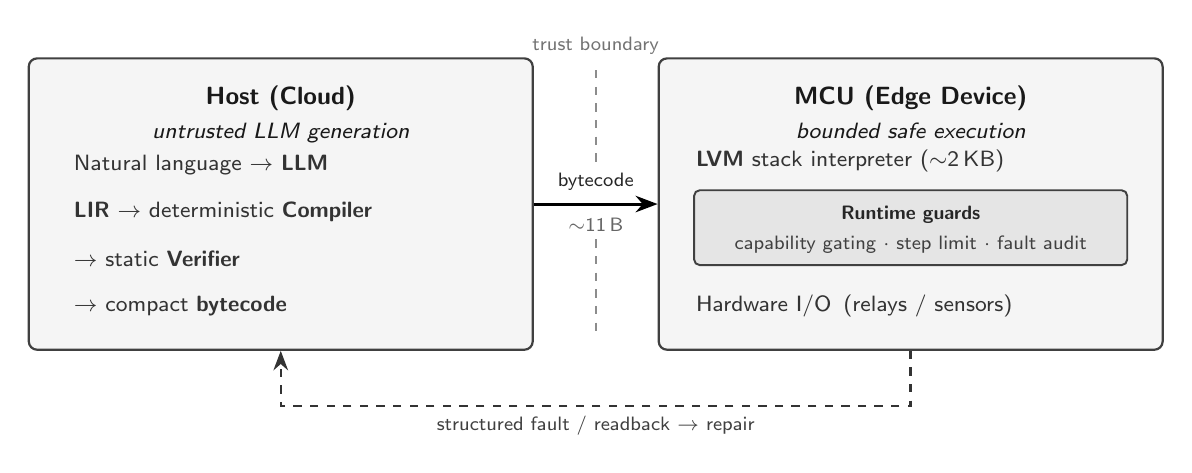
\begin{tikzpicture}[scale=1.0, transform shape,
  >=Stealth, font=\sffamily\small,
  container/.style={draw=black!75, line width=0.8pt, rounded corners=3pt,
                    fill=black!4},
  guard/.style={draw=black!75, line width=0.7pt, rounded corners=2pt,
                fill=black!10},
  title/.style={font=\sffamily\small\bfseries, black!90, align=center},
  item/.style={font=\sffamily\footnotesize, black!80, anchor=west, align=left},
  sub/.style={font=\sffamily\scriptsize, black!60, anchor=west},
  flow/.style={-Stealth, line width=1.1pt, draw=black},
  fb/.style={-Stealth, line width=0.9pt, draw=black!80, dashed},
]

% ============ LEFT CONTAINER: Host / untrusted generation ============
\node[container, minimum width=6.4cm, minimum height=3.7cm] (host) at (3.3, 0) {};
\node[title, anchor=north] at (3.3, 1.62) {Host (Cloud)\\[1pt]\footnotesize\mdseries\itshape untrusted LLM generation};

\node[item] at (0.55, 0.50) {Natural language $\to$ \textbf{LLM}};
\node[item] at (0.55, -0.10) {\textbf{LIR} $\to$ deterministic \textbf{Compiler}};
\node[item] at (0.55, -0.70) {$\to$ static \textbf{Verifier}};
\node[item] at (0.55, -1.30) {$\to$ compact \textbf{bytecode}};

% ============ RIGHT CONTAINER: MCU / bounded execution ============
\node[container, minimum width=6.4cm, minimum height=3.7cm] (mcu) at (11.3, 0) {};
\node[title, anchor=north] at (11.3, 1.62) {MCU (Edge Device)\\[1pt]\footnotesize\mdseries\itshape bounded safe execution};

\node[item] at (8.45, 0.55) {\textbf{LVM} stack interpreter ($\sim$2\,KB)};
% highlighted guard sub-box (the security pitch)
\node[guard, minimum width=5.5cm, minimum height=0.95cm, anchor=center]
  (gbox) at (11.3, -0.30) {};
\node[font=\sffamily\scriptsize\bfseries, black!85, anchor=north] at (11.3, 0.10)
  {Runtime guards};
\node[font=\sffamily\scriptsize, black!75, anchor=north, align=center] at (11.3, -0.28)
  {capability gating $\cdot$ step limit $\cdot$ fault audit};
\node[item] at (8.45, -1.30) {Hardware I/O \,(relays / sensors)};

% ============ FORWARD FLOW: bytecode crosses trust boundary ============
\draw[flow] (host.east) -- (mcu.west)
  node[font=\sffamily\scriptsize, black!85, midway, above=1pt] {bytecode}
  node[font=\sffamily\scriptsize, black!60, midway, below=1pt] {$\sim$11\,B};

% trust boundary: vertical dashed line in the gap, crossed by the bytecode arrow
\draw[black!45, dashed, line width=0.6pt] (7.3, 1.7) -- (7.3, 0.45);
\draw[black!45, dashed, line width=0.6pt] (7.3, -0.45) -- (7.3, -1.7);
\node[font=\sffamily\scriptsize, black!55, anchor=south] at (7.3, 1.78) {trust boundary};

% ============ FEEDBACK LOOP: structured fault / readback -> repair =====
\draw[fb] (mcu.south) -- ++(0,-0.7) -| (host.south)
  node[font=\sffamily\scriptsize, black!75, pos=0.25, below] {structured fault / readback $\to$ repair};

\end{tikzpicture}

  \caption{LIR + LVM system architecture. The two-layer design decouples generation (NL $\to$ LLM $\to$ LIR $\to$ bytecode) from execution (LVM $\to$ hardware I/O), connected by a deterministic compiler with runtime protection mechanisms.}
  \label{fig:architecture}
\end{figure*}

Existing approaches each address only one side of this three-way tension (Fig.~\ref{fig:architecture}). Grammar-constrained decoding~\citep{willard2023structured} ensures that the LLM's output is syntactically well-formed, but provides no runtime safety once the program reaches the device. High-level languages such as Python are easy for LLMs to generate but require a full interpreter (30--300\,KB RAM) with no formal execution boundaries. Compact binary formats such as WebAssembly~\citep{wamr} provide sandboxed execution but need 30--60\,KB RAM (exceeding the budget of most MCUs) and are difficult for LLMs to generate directly. JSON interfaces, the most common LLM output format, produce hundreds of bytes per instruction. No existing approach provides a representation that LLMs can generate reliably, compresses to tens of bytes for transmission, and bounds execution on the device.

We propose a two-layer framework that addresses all three requirements, guided by six design goals defined in Section~\ref{sec:lir_goals}. The first layer is LIR (a structured intermediate representation) that uses a small, C-like grammar oriented toward LLM output. The second layer is compact, varint-encoded bytecode optimized for transmission and on-device execution. A deterministic compiler bridges the two: the LLM generates LIR text, and the compiler lowers it to bytecode with no ambiguity and no information loss.

To make this concrete, consider a task that would be natural in a smart-farm deployment: ``turn on the water pump and read the water level sensor.'' The LLM emits six lines of IR (declaring the required devices, writing a relay, waiting 500\,ms, reading a sensor, and halting). The compiler lowers these to 14 bytes of bytecode. On the MCU, the virtual machine checks that \texttt{relay1} and \texttt{water\_sensor} were explicitly declared before any I/O is allowed, then executes the seven instructions in sequence. If the LLM had hallucinated a write to an undeclared device (e.g., \texttt{relay2}), the capability gate would block it before the pin is touched. If the program contained an infinite loop, the step limit would terminate it after a fixed number of operations. It illustrates the three properties the framework must provide: compact representation (14 bytes for a task that JSON encodes in over a hundred), bounded execution (every I/O gated, every program terminates), and generation stability (a grammar small enough that the LLM rarely deviates). Section~\ref{sec:lir_goals} develops it in full. These design choices also reduce on-device interpretation energy (Section~\ref{sec:res_energy}), which is particularly relevant for battery-constrained edge devices where control-program updates are frequent.

Three technical challenges arise. First, the \emph{generation--execution gap}: LLMs generate structured text well, but compact bytecode is unreadable to models, and the IR-to-bytecode lowering must be deterministic. Second, \emph{on-device bounded execution}: AI-generated programs are untrusted and must be constrained via capability gating, step limits, and structural validation. Third, \emph{closed-loop feedback and repair}: execution failures must produce structured errors that the LLM can use for self-correction. This third challenge is what distinguishes a static code generator from an adaptive edge intelligence agent: the readback--compare--retry mechanism enables the LLM to observe the device's actual state and repair its program accordingly, forming a closed-loop control cycle rather than a fire-and-forget deployment.

Our contributions are as follows:
\begin{itemize}
  \item \textbf{A bounded-execution VM with capability gating and step limits} (Section~\ref{sec:mvm}). The LVM (lightweight virtual machine) is a compact stack machine with a restricted 14-instruction set; its small semantic surface makes determinism, progress, and bounded termination provable by case analysis (Propositions~\ref{thm:determinism}--\ref{thm:bounded}). Because each privileged I/O dispatches through the capability gate, unauthorized access is blocked by a membership test before each I/O rather than by heuristic detection.
  \item \textbf{A two-layer control representation with a deterministic compiler} (Section~\ref{sec:lir}): LIR + bytecode decouples generation friendliness from execution friendliness, with the compiler's termination, determinism, and totality established in Proposition~1 and its consistency with the VM confirmed on 204 verified outputs in Proposition~2.
  \item \textbf{Cross-platform pipeline evaluation} (Section~\ref{sec:evaluation}). The pipeline achieves full pass rate on deterministic tasks and high reliability on random tasks. Best-of-$K$ ($K{=}3$) sampling restores reliability to 0.982 under stochastic generation. The same bytecode and its safety guarantees execute on both ESP8266 (Xtensa) and STM32F103 (ARM Cortex-M3) with fewer than 50 lines of I/O-adapter code changed.
\end{itemize}

The remainder of this paper is organized as follows. Section~\ref{sec:background} frames the design space. Section~\ref{sec:lir} presents the efficiency-driven design: LIR and its compilation to compact bytecode. Section~\ref{sec:mvm} covers the security-driven design: the LVM threat model, bounded executor, capability gating, and static verifier. Section~\ref{sec:formal} formalizes the operational semantics and proves the safety and compiler--VM consistency properties. Section~\ref{sec:security} analyzes each attack surface against those guarantees, and Section~\ref{sec:evaluation} presents the experimental evaluation. Section~\ref{sec:discussion} discusses design trade-offs and scope, and Section~\ref{sec:related} reviews related work. Section~\ref{sec:conclusion} concludes.

% ============================================================
\section{Background and Design Space}
\label{sec:background}

Driving hardware from LLM output involves three layers: (i)~\emph{generation}, where the LLM produces a structured program from natural language; (ii)~\emph{representation}, where that program is encoded for transmission; and (iii)~\emph{execution}, where the encoded program runs on the target device. On resource-constrained MCUs, each layer faces distinct constraints that jointly shape the design space, and no existing representation satisfies all three at once. This section frames those constraints, then surveys how prior work occupies the design space along the generation, representation, and execution axes.

\subsection{Problem Space and Design Axes}
\label{sec:bg_problem}

The three layers translate into three design axes. \emph{Generation friendliness} depends on the surface syntax the LLM must emit: formats abundant in pre-training data (e.g., C-like assignment statements) yield lower error rates than formats rare in pre-training (e.g., raw hexadecimal bytecode or WASM S-expressions). \emph{Payload density} is determined by the representation that travels to the MCU over a potentially bandwidth-constrained link (e.g., 200\,bps on NB-IoT, $\sim$300\,bps on LoRa). Self-describing formats such as JSON carry structural overhead (braces, quotes, and key names) that inflates the payload beyond its semantic content. \emph{Execution safety} depends on what the device can enforce. A microcontroller such as the ESP8266 (Xtensa LX106, 80\,KB RAM) runs firmware in a bare-metal loop with I/O through memory-mapped registers. Because the program originates from an untrusted LLM, the runtime must gate I/O to declared devices, bound execution against infinite loops, and report structured faults for closed-loop repair.

These axes are in tension. Text formats such as JSON generate reliably but are too verbose for the link. Grammar-constrained decoding secures the generation axis but says nothing about execution safety. Dense binary formats execute efficiently but neither generate reliably nor stay within the device memory budget. These tensions exist in any code deployment scenario, but they become critical when LLMs generate control policies for edge systems: the programs must traverse bandwidth-constrained links, execute on MCUs with no OS-level sandboxing, and avoid activation errors with physical safety consequences. Table~\ref{tab:rw_comparison} positions representative approaches along these axes. Each occupies one or two corners. No existing approach is generation-friendly, compact on the wire, and bounded on the device. LIR and its compiled bytecode are designed for exactly this combination.

\begin{table}[t]
\centering
\caption{Design-space positioning of representative approaches and embedded VMs.}
\label{tab:rw_comparison}
\footnotesize
\adjustbox{max width=\columnwidth}{\begin{tabular}{lcccccc}
\toprule
Approach & Gen. & Payload (B) & RAM (KB) & Cap. & Step-lim. & CL \\
\midrule
\multicolumn{7}{l}{\textit{Representative approaches}} \\
JSON + zlib & \checkmark & 106.7 & N/A\textsuperscript{$\dagger$} & \texttimes & \texttimes & \texttimes \\
CBOR & \texttimes & 105.2 & N/A\textsuperscript{$\dagger$} & \texttimes & \texttimes & \texttimes \\
Arduino C & \checkmark & 188.1 & $\sim$30 & \texttimes & \texttimes & \texttimes \\
Grammar-constrained & \checkmark & --- & --- & \texttimes & \texttimes & \texttimes \\
\midrule
\multicolumn{7}{l}{\textit{Embedded VMs}} \\
TinyVM~\citep{tinyvm} & \texttimes & --- & $\sim$1 & \texttimes & \texttimes & \texttimes \\
Darjeeling~\citep{darjeeling} & \texttimes & --- & $\sim$4 & \texttimes & \texttimes & \texttimes \\
MicroPython & \checkmark & $\sim$80--150 & 30--300 & \texttimes & \texttimes & \texttimes \\
AtomVM~\citep{atomvm} & \texttimes & --- & $\sim$16 & \texttimes & \texttimes & \texttimes \\
WAMR (full)~\citep{wamr} & \texttimes & $\sim$50--100 & 30--60 & \texttimes & gas\textsuperscript{$\ddagger$} & \texttimes \\
WAMR (minimal)\textsuperscript{$\S$} & \texttimes & --- & $\sim$15 & \texttimes & gas\textsuperscript{$\ddagger$} & \texttimes \\
WAMR + Outlines & \checkmark\textsuperscript{$\P$} & $\sim$50--100 & 30--60 & \texttimes & gas\textsuperscript{$\ddagger$} & \texttimes \\
\midrule
\textbf{LIR + LVM (this work)} & \checkmark & \textbf{10.9} & $\sim$2\textsuperscript{$\|$} & \checkmark & \checkmark & \checkmark \\
\bottomrule
\end{tabular}}\\[2pt]
{\footnotesize \textsuperscript{$\dagger$}Requires a host-side interpreter; RAM cost is application-dependent. \textsuperscript{$\ddagger$}WAMR provides gas-metering (functionally equivalent to step-limiting) but no application-level capability gating; an authenticated WASM module can access any memory-mapped I/O within its linear memory. \textsuperscript{$\S$}WAMR minimal configuration on ARM Cortex-M (interpreter mode, no JIT); the 15\,KB figure excludes application heap and stack. \textsuperscript{$\P$}With caveats: WAT uses S-expressions with explicit type annotations, more error-prone for LLMs than LIR's C-like syntax; no published data on LLM generation success rate for WAT. \textsuperscript{$\|$}Core VM RAM only; framework overhead depends on platform (see Table~\ref{tab:footprint}).}
\end{table}

\subsection{Structured LLM Generation}
\label{sec:bg_gen}

Grammar-constrained decoding~\citep{willard2023structured} and tools such as Outlines~\citep{outlines} ensure syntactic validity during LLM inference, but they stop at the token boundary: they provide no downstream compilation, no capability declarations, and no bounded execution. A parallel line drives hardware from generated code directly (Python policies for robot arms~\citep{liang2023code}, fine-tuned vision-language models for action output~\citep{brohan2023rt2,openvla}), but these target desktop-class robots rather than MCUs. Recent work extends LLM code generation toward embedded and IoT systems~\citep{esposito2024llm_embedded,liu2023llm4hw}, yet none integrate a generation-targeted IR with formal bounded execution on the device. LIR + LVM targets this gap.

\subsection{Embedded VMs and Their Gaps}
\label{sec:bg_vm}

Lightweight embedded VMs (TinyVM~\citep{tinyvm}, Darjeeling~\citep{darjeeling}, AtomVM~\citep{atomvm}, and WASM/WAMR~\citep{wamr}) provide bytecode interpreters with an emphasis on generality, portability, or sandbox isolation, but none treats LLM generation cost as a design objective. Unlike WASM/WAMR, LIR runs within $\sim$2\,KB RAM while natively expressing capability declarations and readback/retry. Embedded scripting runtimes (MicroPython~\citep{micropython}, eLua~\citep{lua}) need 6--300\,KB and lack capability gating or step-limiting. Composing existing tools, WASM/WAMR for sandboxed execution and grammar-constrained decoding for format validity, leaves three gaps: (1)~WAT is not an LLM-friendly target (S-expressions with explicit type annotations); (2)~WAMR's sandbox offers no application-level capability gating; (3)~the combination provides no integrated closed-loop feedback. Table~\ref{tab:rw_comparison} positions these approaches, showing that the LVM is the only runtime providing both capability gating and step-limit guarantees within a 2\,KB RAM footprint.

Across the three axes above, prior work covers one or two concerns; LIR + LVM is designed to address all three.


% ============================================================
\section{Efficiency-Driven Design: LIR and Compilation}
\label{sec:lir}

\subsection{Two-Layer Representation}
\label{sec:two_layer}

Following Section~\ref{sec:intro}, we adopt a two-layer representation. The first layer is LIR, a structured control representation oriented toward LLM output; the second is a varint-encoded bytecode stream that the compiler generates and the LVM executes. LIR caters to stable generation and ease of debugging; bytecode is optimized for small transmission size and low-overhead execution. A deterministic compiler bridges the two. The overall system architecture is shown in Fig.~\ref{fig:architecture}: a frontend LLM generation pipeline (NL\,$\to$\,LIR\,$\to$\,compiler\,$\to$\,verifier\,$\to$\,bytecode), a backend MCU execution path (transmission\,$\to$\,LVM\,$\to$\,hardware I/O\,$\to$\,feedback\,$\to$\,repair), and a runtime protection layer (capability gating, step-limit, fault audit, closed-loop verification) enforced during execution.

\subsection{LIR Design Goals}
\label{sec:lir_goals}

The system must satisfy six design goals, spanning the representation, the compiler, and the runtime:
\begin{itemize}[nosep,leftmargin=1.5em]
  \item \emph{Representation}: token efficiency (minimal generation cost) and payload density (small transmission size);
  \item \emph{Compiler/verifier}: deterministic compilation (reproducible lowering) and static verifiability (pre-execution checking);
  \item \emph{Runtime}: bounded execution (guaranteed termination) and fault auditability (structured diagnostics).
\end{itemize}
At the LIR level, the representation goals translate to four concrete requirements: LIR must be:

\begin{enumerate}
  \item Smaller than JSON;
  \item Easier to generate and repair than raw hex bytecode;
  \item Deterministically lowerable to bytecode;
  \item Capable of explicitly expressing capability, wait, readback, and retry semantics.
\end{enumerate}

\textbf{Design choices}: LIR adopts C-like assignment statements rather than S-expressions or stack-based representations. This choice is motivated by the abundance of C-like syntax in LLM pre-training data, which benefits stable generation. The one-statement-per-line format facilitates line-by-line normalization and human debugging. \texttt{wait} accepts a millisecond argument to maintain consistency with hardware timing semantics. \texttt{retry} uses a fixed count instead of conditional predicates, trading expressiveness for implementation simplicity. The current statement subset covers deterministic control, temporal sequencing, closed-loop maintenance, and error recovery. Conditional branching is indirectly supported through \texttt{retry}'s implicit readback mechanism.

\textbf{Running example.} Consider the task ``turn on the water pump and read the water level sensor.'' The LLM emits six lines of LIR: first declaring the required devices (\texttt{relay1}, \texttt{water\_sensor}), then issuing a relay write, a 500\,ms delay, a sensor read, and a halt. Each statement maps deterministically to one or two bytecode instructions: capability declarations become \texttt{GTWAY}, writes become \texttt{LIT\,+\,IOW}, reads become \texttt{IOR}, and waits become \texttt{WAIT}. This pattern (declare capabilities, actuate, wait, sense, halt) is the canonical structure of Tasks 1--7 in our deterministic evaluation set (Section~\ref{sec:setup}). The full grammar that defines this mapping is given by the following EBNF:

\begin{lstlisting}[style=mirstyle,caption={LIR EBNF grammar},label={lst:grammar}]
<program>    ::= "task" <identifier> "{" <stmt>+ "}"
<stmt>       ::= <cap_decl> | <set_stmt> | <read_stmt>
               | <wait_stmt> | <halt_stmt>
               | <readback_stmt> | <retry_stmt>
<cap_decl>   ::= "require" "cap" "(" <device> ")"
<set_stmt>   ::= "set" <device> "=" <bit>
<read_stmt>  ::= "read" <device>
<wait_stmt>  ::= "wait" <number> "ms"
<halt_stmt>  ::= "halt"
<readback_stmt> ::= "readback" <device> "expect" <bit>
<retry_stmt> ::= "retry" <number> "times" "{" <stmt>+ "}"
<device>     ::= "water_sensor" | "temperature_sensor"
               | "humidity_sensor" | "relay1" | "relay2"
<bit>        ::= "0" | "1"
<number>     ::= [1-9][0-9]*
\end{lstlisting}

The current grammar subset supports seven statement types (see EBNF grammar). The EBNF grammar enumerates device names explicitly for clarity; a production deployment would use a parameterized \texttt{<identifier>} rule with a separately maintained device registry, enabling new device types without grammar changes. The LLM-generated LIR for the running example is:

\begin{lstlisting}[style=mirstyle,caption={Running example: LLM-generated LIR},label={lst:example}]
task water_pump {
  require cap(relay1)
  require cap(water_sensor)
  set relay1 = 1
  wait 500ms
  read water_sensor
  halt
}
\end{lstlisting}

Device name to device\_id mapping: \texttt{water\_sensor}~(1), \texttt{temperature\_sensor}~(2), \texttt{humidity\_sensor}~(3), \texttt{relay1}~(5), \texttt{relay2}~(6).

\subsection{Compact Bytecode Design Principles}
\label{sec:mbc_principles}

Compact bytecode achieves its small footprint and bounded execution through four design principles, each targeting a distinct constraint of the MCU deployment scenario:

\begin{enumerate}
  \item varint / zigzag encoding for minimal payload size;
  \item a stack-based execution model for deterministic, allocation-free interpretation;
  \item capability-gated I/O for privilege confinement;
  \item a unified fault / pc / steps return format for structured diagnostics.
\end{enumerate}

\subsection{Instruction Set and Bounded-Execution Profile}
\label{sec:instructions}

The LVM is a general-purpose stack machine. Its host-side reference implementation provides roughly fifty instructions spanning control flow, arithmetic, arrays, and debugging (Appendix~\ref{app:full_isa}), but most are unnecessary for deterministic MCU control: categories such as recursion, unbounded loops, dynamic allocation, and division introduce termination or memory behavior that a single step counter cannot bound. For untrusted on-device actuation we therefore deploy a 14-instruction \emph{bounded-execution profile} (Table~\ref{tab:inst_set}): constants and stack manipulation (\texttt{LIT}, \texttt{DUP}, \texttt{DRP}, \texttt{SUB}), equality and control flow for closed-loop retry (\texttt{EQ}, \texttt{JZ}, \texttt{JMP}, \texttt{READBACK}, \texttt{RETRY}), capability-gated I/O (\texttt{GTWAY}, \texttt{IOW}, \texttt{IOR}, \texttt{WAIT}), and termination (\texttt{HALT}). This profile is the subset whose safety properties are formalized in Section~\ref{sec:formal}, deployed to ESP8266 and STM32F103 firmware, and exercised by every experiment in this paper. The remaining instructions are implemented and unit-tested in the host VM but lie outside the on-device safety analysis, for the reasons made precise in Section~\ref{sec:formal_scope}.

\subsection{Encoding Advantages}
\label{sec:encoding}

A fair compression comparison distinguishes \emph{what the LLM generates} (LIR or JSON text) from \emph{what the MCU executes} (compiled bytecode). Table~\ref{tab:encoding} presents four scenarios covering both transmission and execution perspectives.

\begin{table}[t]
\centering
\caption{Fair four-scenario payload comparison (113 tasks, avg.\ bytes).}
\label{tab:encoding}
\footnotesize
\adjustbox{max width=\columnwidth}{\begin{tabular}{llrr}
\toprule
Scenario & LIR side & JSON side & Advantage \\
\midrule
Raw LLM output & 108.0\,B & 285.9\,B & 2.6$\times$ \\
+zlib (level 9) & 86.1\,B & 150.8\,B & 1.8$\times$ \\
Cloud-compiled vs.\ optimized JSON\textsuperscript{$\dagger$} & \textbf{10.9\,B} & 106.7\,B & \textbf{9.8$\times$} \\
Cloud-compiled vs.\ raw-LLM JSON\textsuperscript{$\ddagger$} & 10.9\,B & 150.8\,B & 13.8$\times$ \\
\bottomrule
\end{tabular}}\\[2pt]
{\footnotesize \textsuperscript{$\dagger$} LIR compiled on cloud; JSON uses hand-crafted minimal schema (156.4\,B raw $\to$ 106.7\,B zlib, Appendix Table~\ref{tab:app_json_baseline}). \textsuperscript{$\ddagger$} LIR compiled on cloud; JSON sent as zlib-compressed raw LLM output (285.9\,B $\to$ 150.8\,B).}
\end{table}

Table~\ref{tab:encoding} shows that LIR text is inherently smaller than JSON text (2.6$\times$ raw, 1.8$\times$ after zlib) due to its minimal keyword-based syntax. Under matched optimization, bytecode versus a hand-optimized minimal-schema JSON (156.4\,B raw $\to$ 106.7\,B zlib, Appendix Table~\ref{tab:app_json_baseline}), the ratio is 9.8$\times$, which is the most directly comparable baseline since both sides are optimized. Against zlib-compressed \emph{raw-LLM} JSON (285.9\,B $\to$ 150.8\,B), the advantage grows to 13.8$\times$. Even in the most conservative scenario (raw text without compilation or compression), LIR remains 2.6$\times$ smaller because its grammar removes JSON structural overhead (braces, quotes, key names). Against the binary IoT standard CBOR (105.2\,B, Appendix Table~\ref{tab:app_json_baseline}), the bytecode achieves a 9.6$\times$ compression ratio.

The practical implication is deployment time. On an NB-IoT link at 200\,bps, transmitting 10.9\,B of bytecode takes approximately 0.44\,s, versus 4.27\,s for 106.7\,B of zlib-JSON, a 3.8\,s difference per program. For a field device that receives new control programs periodically (e.g., updated irrigation schedules), this difference determines whether an update completes within a single radio wake window or requires a multi-second connection that drains the battery budget. The 9.8$\times$ ratio is a direct proxy for deployment feasibility on energy-constrained links.

Additional encoding baselines (CBOR: 105.2\,B, MessagePack: 97.42\,B, compact JSON: 127.18\,B) are reported in Appendix~\ref{app:c}. All subsequent analyses use the cloud-compiled scenario (bytecode vs.\ zlib-JSON) as the primary reference, since the two-layer architecture is designed for cloud-to-MCU deployment.

\begin{figure*}[!tbp]
  \centering
  % Fig.2: LIR-to-Bytecode Lowering (two-column before -> after)
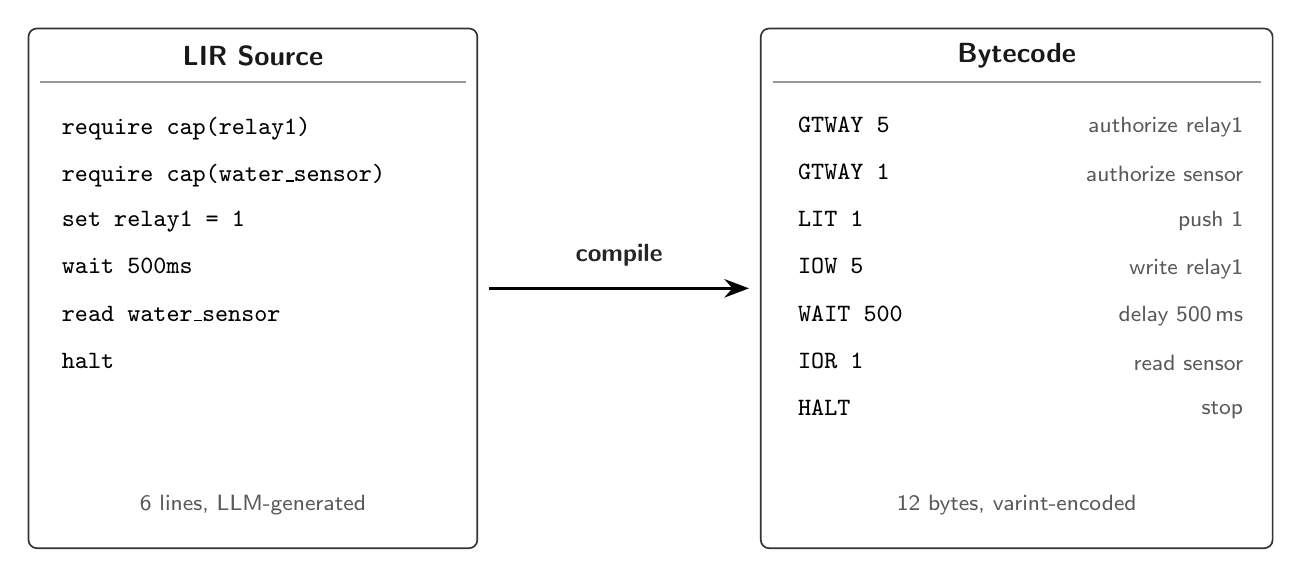
\begin{tikzpicture}[scale=1.0, transform shape,
  >=Stealth, font=\sffamily\normalsize,
  col/.style={draw=black!80, fill=white, line width=0.6pt, rounded corners=3pt},
  code/.style={font=\ttfamily\small, anchor=north west},
  head/.style={font=\sffamily\normalsize\bfseries, black!90},
  note/.style={font=\sffamily\footnotesize, black!65},
]

% ======================= Column 1: LIR Source =======================
\draw[col] (0.0,-3.30) rectangle (5.7,3.30);
\node[head] at (2.85,2.95) {LIR Source};
\draw[black!40] (0.15,2.62) -- (5.55,2.62);
\node[code] at (0.30,2.30) {require cap(relay1)};
\node[code] at (0.30,1.70) {require cap(water\_sensor)};
\node[code] at (0.30,1.10) {set relay1 = 1};
\node[code] at (0.30,0.50) {wait 500ms};
\node[code] at (0.30,-0.10) {read water\_sensor};
\node[code] at (0.30,-0.70) {halt};
\node[note] at (2.85,-2.75) {6 lines, LLM-generated};

% ======================= Column 2: Bytecode =========================
\draw[col] (9.3,-3.30) rectangle (15.8,3.30);
\node[head] at (12.55,2.95) {Bytecode};
\draw[black!40] (9.45,2.62) -- (15.65,2.62);
\node[code] at (9.65,2.30) {GTWAY 5};
\node[code] at (9.65,1.70) {GTWAY 1};
\node[code] at (9.65,1.10) {LIT 1};
\node[code] at (9.65,0.50) {IOW 5};
\node[code] at (9.65,-0.10) {WAIT 500};
\node[code] at (9.65,-0.70) {IOR 1};
\node[code] at (9.65,-1.30) {HALT};
% plain-English glosses for THIS example (value the rule table lacks)
\node[note, anchor=east] at (15.55,2.05) {authorize relay1};
\node[note, anchor=east] at (15.55,1.45) {authorize sensor};
\node[note, anchor=east] at (15.55,0.85) {push 1};
\node[note, anchor=east] at (15.55,0.25) {write relay1};
\node[note, anchor=east] at (15.55,-0.35) {delay 500\,ms};
\node[note, anchor=east] at (15.55,-0.95) {read sensor};
\node[note, anchor=east] at (15.55,-1.55) {stop};
\node[note] at (12.55,-2.75) {12 bytes, varint-encoded};

% ===================== Compile arrow (single) =======================
\draw[-Stealth, line width=1.3pt, black] (5.85,0.0) -- (9.15,0.0);
\node[font=\sffamily\small\bfseries, black!85] at (7.5,0.42) {compile};

\end{tikzpicture}

  \caption{LIR-to-bytecode lowering for the running example.}
  \label{fig:lowering}
\end{figure*}

Fig.~\ref{fig:lowering} illustrates the LIR-to-bytecode lowering for the running example, and Table~\ref{tab:lowering} lists the main lowering relationships for the experimental subset.

\begin{table}[t]
\centering
\caption{Main LIR-to-bytecode lowering rules.}
\label{tab:lowering}
\footnotesize
\begin{tabular}{ll}
\toprule
LIR statement & Lowering result \\
\midrule
\texttt{require cap(relay1)} & \texttt{GTWAY 5} \\
\texttt{require cap(water\_sensor)} & \texttt{GTWAY 1} \\
\texttt{set relay1 = 1} & \texttt{LIT 1 ; IOW 5} \\
\texttt{set relay1 = 0} & \texttt{LIT 0 ; IOW 5} \\
\texttt{set relay2 = 1} & \texttt{LIT 1 ; IOW 6} \\
\texttt{read water\_sensor} & \texttt{IOR 1} \\
\texttt{read temperature\_sensor} & \texttt{IOR 2} \\
\texttt{read humidity\_sensor} & \texttt{IOR 3} \\
\texttt{read relay1} & \texttt{IOR 5} \\
\texttt{wait 500ms} & \texttt{WAIT 500} \\
\texttt{halt} & \texttt{HALT} \\
\bottomrule
\end{tabular}
\end{table}

For \texttt{readback} and \texttt{retry}, the minimal experimental chain is fully implemented and performs real lowering: \texttt{readback} compiles to \texttt{IOR + LIT + EQ}, and \texttt{retry} compiles to explicit control flow composed of \texttt{LIT/DUP/JZ/JMP/SUB/DRP}. The compiler also retains a structured execution-plan output for debugging and subsequent board-level closed-loop runner reuse.

In the formal model \texttt{READBACK} and \texttt{IOR} share identical stack semantics (both push \texttt{dev(d)} given \texttt{d$\in$cap}); in the implementation \texttt{readback} is lowered to \texttt{IOR\,;\,LIT\,;\,EQ} instead of carrying a dedicated opcode, while the structured execution plan retains the ``closed-loop verification read'' intent. This lets fault reports separate a ``sensor read'' from a verification read at the plan level, so the repair loop can identify which stage of the \texttt{set$\to$readback$\to$compare$\to$retry} chain failed.

\subsection{Compiler Properties}
\label{sec:compiler_properties}

Our compiler $\mathcal{C}$ lowers LIR text to bytecode. Let $\text{LIR}^*$ be the set of all valid LIR programs, and $\text{BC}^*$ be the set of all valid bytecode sequences. By design, LIR's EBNF grammar is effectively LL(1) at the token level: each statement starts with a unique keyword, with no left recursion or ambiguity. The only lexer-level ambiguity, the prefix overlap between \texttt{read} and \texttt{readback}, is resolved by the lexer before handing tokens to the parser, leaving the parser itself strictly LL(1). This is a property of the grammar as designed and is realized by the recursive-descent parser in the released implementation. Given it, $\mathcal{C}$'s basic properties follow from standard parser-generator theory (we state them as a design-level property rather than a machine-checked theorem):

\begin{property}[Termination, determinism, and totality]
For every input $p$, $\mathcal{C}$ terminates in $O(n)$ time where $n$ is the token count. Moreover, $\mathcal{C}$ is deterministic ($|\mathcal{C}(p)| = 1$ for all valid $p$) and total, mapping every input (valid or invalid) to either a bytecode sequence or a structured error (\texttt{LIR\_PARSE\_ERROR}).
\end{property}

\textbf{Expression power boundary.}
\label{par:expr_boundary}
The current LIR v0.1 subset covers seven statement types (see EBNF grammar and Table~\ref{tab:lowering}): capability declaration, device set/read, timed wait, halt, readback verification, and retry loops. Constructs outside v0.1 (arbitrary if/else branching, nested loops, general arithmetic, and user-defined functions) and the scalability implications of extending the grammar are discussed in Section~\ref{sec:limitations_detail}.

The compiler establishes only that valid LIR lowers to valid bytecode; it says nothing about bytecode that bypasses the compiler. The compactness secured on the wire must therefore be paired with a static verifier and runtime guards that confine \emph{any} bytecode stream, compiler-produced or adversarial, before it can drive hardware.

% ============================================================
\section{Security-Driven Design: The LVM Bounded Executor}
\label{sec:mvm}

The LVM is the backend that executes untrusted bytecode on the device. Its design is driven by an explicit threat model, which we state first. The remaining subsections then introduce the mechanisms that answer it: a bounded instruction profile, capability gating, step-limiting, and a static verifier.

\subsection{Threat Model}
\label{sec:threat}

We take \emph{runtime bounded execution} as the security scope: an LLM-generated program must not escalate privileges, run unboundedly, or produce an un-audited fault before it can drive hardware. Link encryption, supply-chain integrity, physical tampering, and side-channel attacks (timing, power) are outside the scope of this work, consistent with prior embedded-VM solutions. These are composed from orthogonal mechanisms. We assume the compiler and static verifier are trusted (i.e., they faithfully implement the EBNF grammar and jump-bounds check), and that the MCU hardware and I/O drivers function correctly.

The trusted computing base comprises the static verifier, the LVM executor, the I/O drivers, and the MCU hardware. Everything upstream of the verifier is untrusted: in particular, we treat the LLM and its output as fully adversarial, since a model may hallucinate, be poisoned, or be steered by prompt injection. Defense relies on three complementary layers: (1)~the EBNF parser intercepts format deviations (around 70\% of observed LLM errors); (2)~the static verifier checks opcode validity, varint integrity, and jump-target bounds before any execution; and (3)~the LVM runtime enforces capability gating and step-limits during execution. We consider four threat actors against this stack: \emph{malicious LLM output} (an unauthorized or malformed program), \emph{encoding-layer attacks} (bytecode crafted to bypass the parser entirely), \emph{prompt injection} through the feedback channel, and \emph{side-channel inference} from observable fault behavior. The attack surfaces these actors expose are analyzed against the formal guarantees in Section~\ref{sec:security}.

\subsection{LVM Architecture}
\label{sec:mvm_arch}

The LVM interprets and executes the bytecode on the MCU. The primary implementation targets ESP8266 (Xtensa LX106). Cross-platform validation on STM32F103 (ARM Cortex-M3) confirms platform-independent execution (Section~\ref{sec:stm32}). The LVM state comprises:

\begin{center}
\ttfamily\small
pc / stack / locals / ret-stack / \\
call-depth / steps / fault
\end{center}

and provides a unified response:

\begin{enumerate}
  \item OK: \texttt{[result varint][steps varint][0x01]}
  \item FAULT: \texttt{[fault varint][pc varint][0x00]}
\end{enumerate}

Execution is a single loop over a stack machine. Each iteration first checks the step-limit ($\textit{steps} \geq L$) and the stack bound, then fetches the opcode at \texttt{pc}, increments the step counter, dispatches on the opcode, and advances \texttt{pc} (or redirects it for \texttt{JMP}/\texttt{JZ}). The loop has no recursion and no heap allocation: the operand stack is a fixed-size array, locals are a fixed slot vector, and every operation either pushes/pops a bounded number of slots or performs one capability-checked I/O. This structure lets the same $\sim$430-line core run unmodified on both an 80\,KB-RAM Xtensa device and a 10\,KB-RAM Cortex-M3, with only the GPIO/sensor adapter changed. Every exit is either the OK response (top-of-stack result and consumed step count) or the FAULT response (structured fault code and faulting \texttt{pc}), so the host can always distinguish ``ran to completion'' from ``stopped by a guard'' and feed the latter into the repair loop (Section~\ref{sec:pipeline}).

The quantified resource footprint of the LVM is summarized in Table~\ref{tab:footprint}.

\begin{table}[t]
\centering
\caption{LVM resource footprint (measured on ESP8266 and STM32F103).}
\label{tab:footprint}
\footnotesize
\adjustbox{max width=\columnwidth}{\begin{tabular}{p{3.2cm}ccp{3.5cm}}
\toprule
Metric & ESP8266 & STM32F103C6 & Measurement method \\
\midrule
Flash (LVM core / with framework\textsuperscript{$\dagger$}) & $\sim$4\,KB / --- & $\sim$4\,KB / $\sim$21\,KB & Arduino IDE compilation \\
RAM (stack + vars) & \textbf{$\sim$2\,KB} & \textbf{$\sim$2.7\,KB} & Build report + runtime watermarking \\
Max stack depth & 16 levels & 64 levels & Deepest nested test \\
Code lines (C++) & $\sim$430 & $\sim$430 & Shared core, platform I/O adapters \\
WAMR min config & 30--60\,KB & --- & WAMR documentation~\citep{wamr} \\
\bottomrule
\end{tabular}}\\[2pt]
{\footnotesize \textsuperscript{$\dagger$}STM32F103C6 has 32\,KB flash. The 21\,KB figure includes LVM core logic ($\sim$4\,KB) plus STM32duino framework overhead and DHT sensor library; the LVM core logic itself is identical across platforms. RAM is measured via the build report (.data+.bss) and runtime stack watermarking.}
\end{table}

\subsection{Static Verifier}
\label{sec:validator}

The host-side static verifier is the first line of defense: it rejects malformed bytecode before transmission, so a faulty stream never consumes device bandwidth or execution cycles. Verification proceeds in two passes over the decoded instruction stream. The first pass reconstructs instructions from the varint encoding and rejects any byte sequence that does not decode to a known opcode carrying a well-formed operand; an unsupported opcode, a truncated varint, or a device identifier outside the valid range each aborts decoding with a bad-encoding fault. The second pass examines the control-flow skeleton: every jump offset is resolved to an absolute target, and a target that falls outside the program bounds is rejected. Resolving jumps statically guarantees that the program counter cannot leave the loaded program once execution begins, which removes an entire class of out-of-bounds behavior from the runtime. Because both passes complete on the host before the payload is sent, the device receives only bytecode whose opcodes decode and whose jumps land in range, leaving the runtime guards to handle the faults that depend on execution state rather than on structure.

\subsection{Runtime Protection Mechanisms}
\label{sec:safety}

The runtime guards handle the faults that static verification cannot anticipate, because they depend on values the program computes as it runs. Four guards operate during the execution loop, each confining a distinct fault class. Capability gating is the central mechanism: the LVM admits a device into an authorization set only when an explicit gateway instruction names it, and every subsequent write or read checks membership in that set before touching hardware. An I/O to a device that was never authorized raises a capability fault instead of driving the pin, so the capability gate blocks unauthorized access via a membership test before each I/O rather than by heuristically detecting suspicious patterns after the fact. The step-limit guard bounds total work: the counter advances by one per instruction and, on reaching the limit $L$, forces termination, so a backward jump or a retry loop either converges within a finite number of steps or stops safely at the bound. The stack guard rejects both an overflow that would exceed the fixed operand-stack capacity and an underflow that would pop an empty stack, the latter being the typical symptom of a truncated or adversarial program. A program-counter bound complements the verifier's static jump check by catching any residual out-of-range fetch at runtime. When a guard fires, it returns a structured fault carrying the fault class and the faulting program counter rather than failing silently. This keeps the runtime safe to expose to untrusted output, and gives the repair loop (Section~\ref{sec:pipeline}) a precise signal to act on.

Capability gating also provides a form of structural privacy. \textbf{Structural privacy of generated programs.} It bounds not only what a program can activate but also what it can leak. A concern specific to LLM-based edge intelligence is that LLMs can memorize and reproduce sensitive training data such as credentials or secrets~\citep{carlini2021extracting}. In our setting this surface is structurally narrow: LIR programs cannot express free-form strings or secrets, since the grammar (Listing~\ref{lst:grammar}) admits only a fixed device vocabulary, bit values, and integer durations, and the compiler rejects any token outside this alphabet. A leaked credential therefore cannot survive compilation to bytecode, and capability gating further bounds the \emph{effect} of any generated program to the declared device set. What LIR does \emph{not} address is leakage in the natural-language prompt or in the LLM's hidden state, nor confidentiality of the bytecode in transit (link encryption is out of scope); these are orthogonal protections that compose with LIR rather than being subsumed by it.

The complete instruction set for the experimental subset is listed in Table~\ref{tab:inst_set}, with each instruction's opcode, operands, stack effect, and step count.

\begin{table}[t]
\centering
\caption{Compact bytecode instruction set (14-instruction formalized subset).}
\label{tab:inst_set}
\footnotesize
\adjustbox{max width=\columnwidth}{\begin{tabular}{lllll}
\toprule
Instr. & Opcode & Operand & Stack effect & Steps \\
\midrule
\texttt{LIT} & 0x1e & value (svarint) & push value & 1 \\
\texttt{GTWAY} & 0x50 & 1B dev\_id & --- & 1 \\
\texttt{IOW} & 0x46 & 1B dev\_id & pop, write & 1 \\
\texttt{IOR} & 0x47 & 1B dev\_id & push read & 1 \\
\texttt{WAIT} & 0x51 & ms (uvarint) & --- & 1 \\
\texttt{HALT} & 0x52 & --- & --- & 1 \\
\texttt{EQ} & 0x2c & --- & pop a,b; push (a==b) & 1 \\
\texttt{JZ} & 0x65 & offset (svarint) & pop, jmp if 0 & 1 \\
\texttt{JMP} & 0x64 & offset (svarint) & --- & 1 \\
\texttt{DUP} & 0x40 & --- & push top & 1 \\
\texttt{SUB} & 0x33 & --- & pop a,b; push (b-a) & 1 \\
\texttt{DRP} & 0x41 & --- & pop, discard & 1 \\
\texttt{READBACK}\textsuperscript{$\dagger$} & (lowered) & 1B dev\_id & push dev state & 1 \\
\texttt{RETRY}\textsuperscript{$\dagger$} & (lowered) & count, offset & dec counter; jmp if $>$0 & 1 \\
\bottomrule
\end{tabular}}\\[2pt]
{\footnotesize \textsuperscript{$\dagger$}\texttt{READBACK} and \texttt{RETRY} are logical instructions of the formal model (Section~\ref{sec:formal}); the compiler lowers them to sequences over the twelve primitive opcodes above (\texttt{readback}\,$\to$\,\texttt{IOR\,;\,LIT\,;\,EQ}; \texttt{retry}\,$\to$ a \texttt{LIT/DUP/JZ/JMP/SUB/DRP} loop), so they carry no dedicated bytecode opcode. Operand widths are variable-length: unsigned args use uvarint, while \texttt{LIT} values and jump offsets use zigzag-encoded svarint.}
\end{table}

Each instruction consumes exactly one step: the LVM increments the step counter by~1 for every instruction executed, triggering a fault when $k \geq L$. For program instruction count $n$, actual execution steps are $\leq \min(n, L)$; loops composed of \texttt{JZ}/\texttt{JMP} or \texttt{RETRY} still increment $k$ per iteration, so they either terminate within finite steps or raise a step-limit fault. With the runtime guards in place, we now analyze how they respond to each attack surface.

\section{Formal Safety Guarantees}
\label{sec:formal}

This section establishes three safety properties of the LVM execution model (determinism, progress, and bounded termination) and the consistency between a compiled program and its execution. Because the LVM restricts itself to 14 fixed-step instructions (no unbounded loops, no dynamic allocation, no instruction whose cost depends on its operands), each property reduces to case analysis over a finite rule set and a monotone step counter. The formalization follows a small-step operational style; the complete machine configuration, 17 transition rules, and full proofs are given in Appendix~\ref{app:rules}--\ref{app:proofs}.

\subsection{Execution Model}
\label{sec:config}

We model LVM execution as a state transition system. A configuration $\sigma = \langle p,\, pc,\, s,\, \mathit{dev},\, \mathit{cap},\, k,\, L,\, f,\, r \rangle$ comprises the bytecode program $p$, program counter $pc$, operand stack $s$, device state $\mathit{dev}$, capability set $\mathit{cap}$, step counter $k$, step limit $L$, fault status $f$, and retry counter $r$. Every instruction advances $k$ by~1; when $k \geq L$, the \textsc{StepGuard} rule forces a \texttt{STEP} fault. I/O instructions (\texttt{IOW}, \texttt{IOR}, \texttt{READBACK}) check $d \in \mathit{cap}$ before dispatching; if the check fails, a \texttt{CAP} fault is raised. Invalid opcodes trigger an \texttt{OPC} fault. The full 17-rule transition system is closed over the 14-instruction set of Table~\ref{tab:inst_set}.

\subsection{Safety Properties}
\label{sec:theorems}

We establish three properties that together guarantee the LVM cannot harm the device it controls. In plain terms: the VM always terminates (it cannot run forever), every I/O is checked against a declared allow-list (it cannot touch unauthorized hardware), and the same program always produces the same result (execution is predictable). These properties hold because the instruction set is deliberately restricted: every instruction costs exactly one step, there is no unbounded loop instruction, and every I/O goes through a capability check. The formal statements follow.

\begin{proposition}[Determinism]
\label{thm:determinism}
For any configuration $\sigma$, if $\sigma \xrightarrow{1} \sigma_1$ and $\sigma \xrightarrow{1} \sigma_2$, then $\sigma_1 = \sigma_2$.
\end{proposition}

\begin{proposition}[Progress]
\label{thm:progress}
For every non-terminal configuration $\sigma$ with $f = \bot$ and $k < L$, there exists $\sigma'$ such that $\sigma \xrightarrow{1} \sigma'$.
\end{proposition}

\begin{proposition}[Bounded execution]
\label{thm:bounded}
Starting from $\sigma_0 = \langle p, 0, \epsilon, \mathit{dev}_0, \mathit{cap}_0, 0, L, \bot, r_0 \rangle$: (1)~$\sigma_0$ reaches a terminal configuration in at most $L$ steps; (2)~any $\texttt{IOW}\;d$ or $\texttt{IOR}\;d$ with $d \notin \mathit{cap}$ triggers a \texttt{CAP} fault; (3)~any invalid opcode triggers an \texttt{OPC} fault; (4)~the retry counter $r$ is strictly decreasing per loop iteration, and total execution steps remain bounded by $L$.
\end{proposition}

\noindent Intuitively: (1) holds because every rule increments $k$ by exactly~1, so \textsc{StepGuard} forces termination within $L$ steps; (2)--(3) hold because the first unauthorized I/O or invalid opcode immediately raises its fault; (4) holds because each retry iteration decrements $r$ while $k$ keeps rising. Complete proofs are in Appendix~\ref{app:proofs}.

Proposition~\ref{thm:bounded}(2)--(3) has a direct practical consequence for the security metric used in the evaluation. We define the Unauthorized Access Blocking Rate (UABR) as the fraction of unauthorized I/O requests that are blocked before reaching hardware. Within the formal model, this rate is exactly~1: every unauthorized request is caught by the capability check, with no dependence on how the program was generated.

\begin{corollary}[UABR lower bound, within the model]
\label{prop:uabr}
Under the threat model (Section~\ref{sec:threat}), every unauthorized request raises a \texttt{CAP} fault, so $\text{UABR}(r) = 1$ at the model level. This follows directly from Proposition~\ref{thm:bounded}(2)--(3). The empirical UABR in Section~\ref{sec:res_e2} measures the implementation's agreement with this model-level bound.
\end{corollary}

\noindent This bound is a direct consequence of checking $d \in \mathit{cap}$ before each \texttt{IOW}/\texttt{IOR}/\texttt{READBACK}, not an emergent property: it holds independent of whether the generating LLM is honest, hallucinating, or adversarial, and carries over to the synthetically adversarial payloads of Section~\ref{sec:res_fuzzing}, which never pass through the LLM at all.

\subsection{Compiler--VM Consistency}
\label{sec:consistency}

The safety properties above bound what the LVM does with \emph{any} bytecode. Consistency closes the loop back to the compiler of Section~\ref{sec:lir}, establishing that a compiled program executes with the semantics its LIR source intended.

\begin{property}[Compiler--VM consistency]
\label{prop:consistency}
For each grammar production in the LIR EBNF, the lowering rule of Table~\ref{tab:lowering} preserves the intended semantics. By case analysis over the seven statement types (full analysis in Appendix~\ref{app:proofs}), each lowering is a direct structural encoding of its EBNF production: e.g., \texttt{set $d$ = $v$} lowers to \texttt{LIT $v$ ; IOW $d$}, where rule \textsc{Lit} pushes $v$ and rule \textsc{Iow-Ok} writes it to $\mathit{dev}(d)$; \texttt{retry $n$ times} lowers to a loop with decreasing counter $r$, where rules \textsc{Retry-Loop}/\textsc{Retry-Exhaust} guarantee exactly $n$ iterations. Full-program equivalence $\llbracket p \rrbracket_{\text{LIR}} = \llbracket \mathcal{C}(p) \rrbracket_{\text{LVM}}$ follows by induction on the statement sequence, using the \emph{stack-balance invariant}: every statement-level lowering leaves the operand stack at the same height it found it, so sequential composition preserves both device state $\mathit{dev}$ and capability set $\mathit{cap}$ across statement boundaries. This is a hand proof over a fixed seven-production grammar, corroborated empirically: across 204 verified compiler outputs (113 deterministic + 91 verified closed-loop outputs, Appendix Table~\ref{tab:app_closed_loop}) the LVM device state matches the expected effect in every case.
\end{property}

\subsection{Scope}
\label{sec:formal_scope}

The formal model covers the 14 instructions of the bounded-execution profile (Table~\ref{tab:inst_set}), which is exactly the subset deployed to firmware and exercised by the evaluation. The broader instruction categories of the host VM (Appendix~\ref{app:full_isa}), namely functions and recursion, general loops, dynamic memory, and division, are excluded because each introduces behavior that a single step counter cannot bound. The LIR v0.1 grammar restricts generation to the same subset, so the representation, firmware, and formal model coincide on one bounded surface. The three properties follow from two design choices, a finite fixed-step instruction set and a capability check before each I/O, and the complete proofs are in Appendix~\ref{app:proofs}.

\subsection{Closed-Loop and Host VM}
\label{sec:closed_loop}

The current system supports the closed-loop chain \texttt{set $\to$ readback $\to$ compare $\to$ retry}, giving the LLM a unified observation-and-repair interface. At runtime the LVM follows a fixed five-stage path (loading, decoding, static checking, runtime guarding, and output) in which any guard violation transitions immediately to a terminal Fault state. Fig.~\ref{fig:fsm} illustrates the closed-loop verification state machine.

\begin{figure*}[tp]
  \centering
  % Fig.4: Closed-Loop FSM — auto-generated
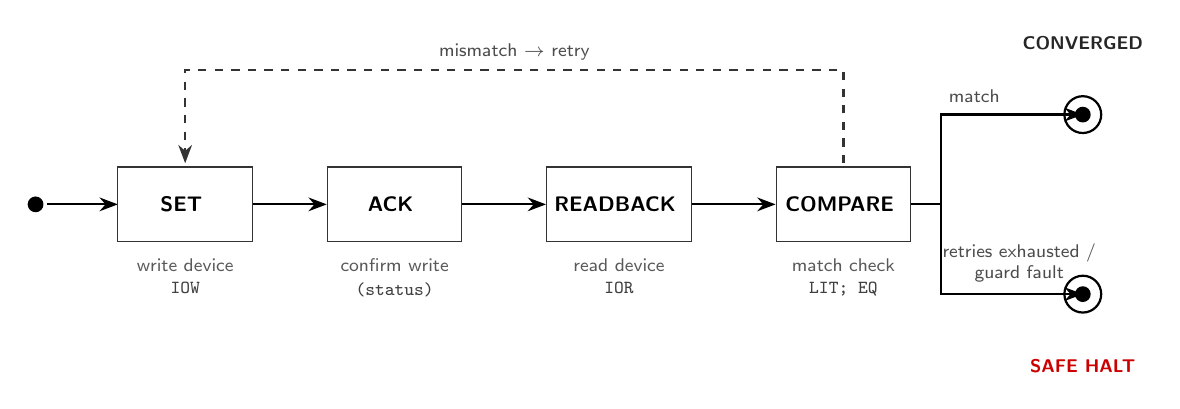
\begin{tikzpicture}[scale=0.95, transform shape,
  >=Stealth, font=\sffamily\small,
  state/.style={draw=black!80, fill=white, minimum width=1.8cm,
                minimum height=1.0cm, align=center, inner sep=3pt,
                font=\sffamily\footnotesize\bfseries},
  arr/.style={-Stealth, thick, draw=black},
  darrow/.style={-Stealth, thick, draw=black!80, dashed},
]

% Initial state
\fill[black] (-2.00, 0.00) circle (3pt);
\draw[arr] (-1.85, 0.00) -- (-0.90, 0.00);

% States
\node[state] (set) at (0.00, 0.00) { SET };
\node[state] (ack) at (2.80, 0.00) { ACK };
\node[state] (read) at (5.80, 0.00) { READBACK };
\node[state] (cmp) at (8.80, 0.00) { COMPARE };

% Annotations
\node[font=\sffamily\scriptsize, black!65, anchor=north] at (0.00, -0.60) {write device};
\node[font=\sffamily\scriptsize, black!65, anchor=north] at (2.80, -0.60) {confirm write};
\node[font=\sffamily\scriptsize, black!65, anchor=north] at (5.80, -0.60) {read device};
\node[font=\sffamily\scriptsize, black!65, anchor=north] at (8.80, -0.60) {match check};

% LVM instruction mapping
\node[font=\ttfamily\scriptsize, black!75, anchor=north] at (0.00, -0.92) {IOW};
\node[font=\ttfamily\scriptsize, black!75, anchor=north] at (2.80, -0.92) {(status)};
\node[font=\ttfamily\scriptsize, black!75, anchor=north] at (5.80, -0.92) {IOR};
\node[font=\ttfamily\scriptsize, black!75, anchor=north] at (8.80, -0.92) {LIT; EQ};

% State transitions
\draw[arr] (set.east) -- (ack.west) ;
\draw[arr] (ack.east) -- (read.west) ;
\draw[arr] (read.east) -- (cmp.west) ;

% CONVERGED terminal (match)
\fill[black] (12.00, 1.20) circle (3pt);
\draw[line width=0.8pt] (12.00, 1.20) circle (7pt);
\draw[arr] (cmp.east) -- ++(0.4, 0) |- (12.00, 1.20);
\node[font=\sffamily\scriptsize, black!70, anchor=south] at (10.55, 1.24) {match};
\node[font=\sffamily\scriptsize\bfseries, black!85, anchor=south] at (12.00, 1.95)
  {CONVERGED};

% SAFE-HALT terminal (retries exhausted / guard fault)
\fill[black] (12.00, -1.20) circle (3pt);
\draw[line width=0.8pt] (12.00, -1.20) circle (7pt);
\draw[arr] (cmp.east) -- ++(0.4, 0) |- (12.00, -1.20);
\node[font=\sffamily\scriptsize, black!70, anchor=south, align=center] at (11.15, -1.16)
  {retries exhausted /\\ guard fault};
\node[font=\sffamily\scriptsize\bfseries, red!80!black, anchor=north] at (12.00, -1.95)
  {SAFE HALT};

% Retry loop (routed over the top to avoid the bottom annotations)
\draw[darrow]
  (8.80, 0.55)
  |- (0.00, 1.80)
  -| (0.00, 0.55);
\node[font=\sffamily\scriptsize, black!70, anchor=south] at (4.40, 1.80)
  {mismatch $\rightarrow$ retry};

\end{tikzpicture}
  \caption{State-machine model of closed-loop verification.}
  \label{fig:fsm}
\end{figure*}

\begin{rmk}[Running example revisited]
For the running example introduced in Section~\ref{sec:intro} and compiled in Section~\ref{sec:lir_goals} (``turn on the water pump and read the water level sensor''), the compiled 7-instruction sequence executes in 7 steps. With the default step limit $L=1000$, this consumes only 0.7\% of the budget, illustrating that the theoretical bound (Proposition~\ref{thm:bounded}) provides a $>\!140\times$ safety margin over typical benign programs. This margin is by design: the step limit protects against adversarial programs, not typical ones.
\end{rmk}

% ============================================================
\section{Security Analysis}
\label{sec:security}

We now reason through each attack surface exposed by the threat model, showing how the runtime guards and formal guarantees mitigate them. The empirical validation (per-guard ablation and an 8{,}000-payload fuzzing campaign) follows in Section~\ref{sec:exp2}.

\subsection{Attack Surfaces and Defenses}
\label{sec:attack_surfaces}

\noindent\textbf{Unauthorized activation.} An adversary may try to drive a relay or pump the operator never authorized, the most consequential attack on physical hardware. Each \texttt{IOW}/\texttt{IOR}/\texttt{READBACK} dispatches through the capability gate: if the target device is absent from the declared set $\mathit{cap}$, the rule raises a \texttt{CAP} fault and the configuration becomes terminal before a write reaches the driver. Proposition~\ref{thm:bounded}(2) makes this independent of the input source: an unauthorized access raises a \texttt{CAP} fault whether or not the program was generated honestly. This is the basis of the $\text{UABR}=1$ lower bound (Corollary~\ref{prop:uabr}).

\noindent\textbf{Invalid and injected opcodes.} A malformed or hostile stream may contain bytes that decode to no valid instruction. The static verifier rejects such streams before execution. Any opcode that nonetheless reaches the interpreter triggers the \textsc{OpcF} rule and an \texttt{OPC} fault (Proposition~\ref{thm:bounded}(3)). The two layers are deliberately redundant: structurally malformed bytecode is caught statically, while a decodable-but-invalid opcode is caught at runtime.

\noindent\textbf{Non-terminating execution.} An adversary may craft backward jumps or retry loops intended to cause non-termination or exhaust device resources. Because every rule, including \texttt{JMP}, \texttt{JZ}, and \texttt{RETRY}, increments the step counter $k$ by exactly one, \textsc{StepGuard} forces a \texttt{STEP} fault after at most $L$ steps (Proposition~\ref{thm:bounded}(1)). The bound is on steps executed rather than on the program's syntactic shape, so it holds regardless of how the control flow is arranged. On a microcontroller wired to physical actuators, this converts a potential stuck-actuator incident into a clean, audited halt.

\noindent\textbf{Malformed encoding.} An adversary may craft a bytecode stream with truncated varints, out-of-bounds jump targets, or stack-violating sequences. The static verifier intercepts structurally malformed bytecode before transmission. Any decodable-but-invalid stream that reaches the runtime triggers the \textsc{PopF} rule or stack-bound checks. Because the two layers cover structurally malformed and decodable-but-invalid streams respectively, no adversarial stream can bypass both.

\noindent\textbf{Adversarial instructions and prompt injection.} LLM-based edge intelligence exposes two injection surfaces: the natural-language prompt itself and the closed-loop feedback channel. An attacker may embed malicious directives in the user instruction (e.g., instructing the LLM to write to an unauthorized device or enter an infinite loop), or inject adversarial sensor values or fault text through the feedback path to steer subsequent generation. LIR + LVM mitigates the \emph{consequence} of both vectors through defense-in-depth. The EBNF grammar constrains the LLM's output to a fixed alphabet of statements (set/read/wait/halt/retry on declared device names), so a semantically malicious instruction cannot survive compilation if it requires constructs outside the grammar. The static verifier rejects malformed bytecode before transmission. Capability gating ensures that even a syntactically valid but adversarial program cannot access undeclared devices. The step limit bounds total execution regardless of control-flow arrangement. The key property is that each layer operates on a different artifact (source text, bytecode structure, runtime state), so bypassing one layer does not bypass the others. A prompt-injection attack that succeeds at the LLM level, convincing the model to emit a malicious but syntactically valid program, still faces the same capability and step-limit guarantees as any other untrusted program (Corollary~\ref{prop:uabr}). What the architecture does \emph{not} defend against is a prompt injection that causes the LLM to emit a syntactically valid, capability-compliant program with \emph{incorrect semantics} (e.g., writing~1 to a relay when the user intended~0); this class of attack requires semantic validation beyond the VM's scope.

\noindent\textbf{Side-channel inference.} The LVM returns a unified fault format (fault code, program counter, status byte) regardless of which guard fired, so an observer cannot distinguish the fault class from the response shape alone. Timing and power side channels are out of scope.

\noindent\textbf{Physical-safety boundary.} UABR measures blocking of unauthorized VM-level access requests; it does not imply physical safety. A single \emph{authorized} \texttt{IOW} instruction can still activate a pump or relay, so physical safety requires external hardware interlocks (watchdog timers, current limiters) beyond the VM's scope. The guarantee is that the set of \emph{possible} actuations is bounded to the declared capability set, not that every authorized actuation is physically benign.

The qualitative arguments above are validated empirically in the next section, where a per-guard ablation and an 8{,}000-payload fuzzing campaign stress the combined boundary across the attack classes enumerated here.

% ============================================================
\section{Evaluation}
\label{sec:evaluation}

Our evaluation answers four questions, aligned with the security and efficiency axes that motivate this work:
\begin{itemize}[nosep]
  \item \textbf{Q1 (Efficiency):} How small is the LIR/bytecode representation relative to JSON, CBOR, and Arduino~C, across transmission payload, generation tokens, and on-device execution energy (Section~\ref{sec:exp1})?
  \item \textbf{Q2 (Security):} Does the LVM contain the output of an untrusted LLM (or an adversary), and does each guard contribute independently (Section~\ref{sec:exp2})?
  \item \textbf{Q3 (Reliability):} How reliably does the pipeline generate correct programs across temperatures, models, and task complexities, and on tasks derived from real-world IoT deployments (Section~\ref{sec:exp3reliability})?
  \item \textbf{Q4 (Portability):} Does the same bytecode and its safety guarantees execute unchanged across MCU architectures (Section~\ref{sec:stm32})?
\end{itemize}
We address them in turn, with the experimental setup common to all of them described next.

\subsection{Experimental Setup}
\label{sec:setup}

\textbf{LLM.} All experiments used LLaMA~3.1~8B~\citep{dubey2024llama} as the primary model, served via Ollama on a local server. Multi-model comparison (Appendix~\ref{app:c}, Table~\ref{tab:app_model_compare}) additionally evaluated Qwen3~8B and DeepSeek-R1~8B~\citep{guo2024deepseek} as local models, and DeepSeek-V4-Pro via commercial API to validate cross-architecture generalization. Temperature settings varied by experiment: temperature\,=\,0.0 for deterministic baselines, 0.0--1.0 for temperature scanning. Apart from temperature, all sampling parameters were left at the Ollama defaults (top-p 0.9, top-k 40, repetition penalty 1.1); only the temperature was set explicitly, and no fixed random seed was pinned for LLM generation. Consequently, temperature\,$>$\,0 runs are not bit-for-bit reproducible; we therefore report the mean and standard deviation over three independent passes for every stochastic setting (Table~\ref{tab:temperature}).

\textbf{Hardware.} The primary MCU target was ESP8266 (80\,KB RAM, Xtensa LX106) running Arduino framework. The LVM firmware ($\sim$430 lines C++, $\sim$2\,KB RAM) was compiled via Arduino IDE. Cross-platform validation was performed on STM32F103C6T6 (ARM Cortex-M3, 32\,KB flash, 10\,KB RAM) using the STM32duino board package, confirming that LVM's platform-independent C++ core requires only I/O adapter changes ($<$50 lines) for porting. End-to-end LLM generation experiments were conducted on ESP8266. STM32 validation confirmed correct execution of compiled bytecode (capability-gated I/O, sensor reads, relay control) via serial communication.

\textbf{Task sets.} We used five task sets (all included in the repository; see the data availability statement): (1)~113 deterministic tasks covering 7 control patterns; (2)~96 closed-loop tasks covering 12 categories; (3)~15 control-flow tasks (if/else, repeat); (4)~600 randomly generated tasks across 12 categories (50 per category); (5)~29 tasks derived from real-world IoT deployments (Home Assistant, Tasmota, ESPHome, Arduino/ESP projects) covering 20 control pattern categories.

\textbf{Metrics.} We evaluated using the following metrics, defined formally to ensure reproducibility:

\emph{Compression ratio}:
\[
\begin{gathered}
R_{\text{AVG}} = \frac{1}{|T|} \sum_{t \in T} \frac{B_{\text{JSON}}(t)}{B_{\text{compact}}(t)}, \\[4pt]
R_{\text{WEIGHTED}} = \frac{\sum_{t} B_{\text{JSON}}(t)}{\sum_{t} B_{\text{compact}}(t)}.
\end{gathered}
\]

\emph{Task Success Rate (TSR)}:
\[
\text{TSR} = \frac{1}{|T|} \sum_{t \in T} \mathbf{1}[\,t \text{ passes all stages}\,],
\]
with 95\% Wilson confidence intervals.

\emph{Unauthorized Access Blocking Rate (UABR)}: $\text{UABR} = N_{\text{blocked}} / N_{\text{total}}$, where $N_{\text{blocked}}$ is the number of unauthorized requests blocked by capability gating or the validator.

\emph{Safe Convergence Rate (SCR)}: the fraction of tasks reaching the target state after $k$ retry rounds.

\emph{First-success@k}: the fraction of tasks whose first successful generation occurs at round $k$ (non-cumulative; distinguishes from pass@k which is cumulative).

\textbf{Experiment overview.} We organized experiments along three axes:
\begin{itemize}[nosep,leftmargin=1.5em]
  \item \textbf{(A) Efficiency}: compression ratio and RTT of bytecode vs.\ JSON.
  \item \textbf{(B) Security}: effectiveness of capability gating, step-limit, validator, and fault audit (UABR, fault distribution, SAFE shunting).
  \item \textbf{(C) Reliability}: whether the LLM$\to$LIR$\to$bytecode pipeline produces correct programs, evaluated on 113 deterministic tasks covering seven control patterns (single write, single read, write-then-wait-then-halt, wait-then-read, write-wait-read, multiple reads, and pulse).
\end{itemize}

\textbf{Core results (temperature,=,0.0).} On the 113-task set, each pipeline stage (IR validity, compilation, verification, execution, and task success) achieved 1.000 (95\% Wilson CI: [0.967, 1.000]). Of the 113 tasks, 100 required no repair, and the remaining 13 were corrected in the second round, with no failures.

\textbf{Additional experiments.} We evaluate three further dimensions (detailed results in Appendix~\ref{app:c}): (i)~\emph{Closed-loop control}: retry raises SCR under both paths, and the LIR path achieves lower RTT than JSON under the same retry strategy. (ii)~\emph{Token cost}: LIR reduces output tokens by 51\% versus JSON; under prompt caching, its incremental cost is roughly half of JSON's (Table~\ref{tab:gen_results}). (iii)~\emph{Random task coverage}: on 600 randomly generated tasks, the success rate is 0.970, with 7 of 12 categories achieving 100\% (Section~\ref{sec:res_random}). (iv)~\emph{Arduino~C baseline}: LLM-generated Arduino~C produces 17.3$\times$ larger payloads than the bytecode.

Fig.~\ref{fig:forest_rates} consolidates the headline success rates and their 95\% Wilson confidence intervals across all task sets, so the relative precision of each estimate (driven by sample size) can be read at a glance: the large deterministic and random sets yield tight intervals, while the smaller real-world and closed-loop subsets carry wider ones.

\intextfig{width=\columnwidth}{Fig11_forest_rates.pdf}{Headline success rates with 95\% Wilson confidence intervals across all task sets (forest plot).}{fig:forest_rates}

\subsubsection{Pipeline and Repair Strategy}
\label{sec:pipeline}

The complete generation chain is:

\[
\adjustbox{max width=\columnwidth}{$\displaystyle
\text{NL} \to \lir{} \to \text{Compiler} \to \text{Verifier} \to \lvm{}/\text{Sim} \to \text{Feedback} \to \text{Repair}
$}
\]

Taking the running example from Section~\ref{sec:intro} (``turn on the water pump and read the water level sensor''): the LLM outputs 6 lines of LIR, the compiler lowers it to 14 bytes of bytecode (\texttt{GTWAY 5; GTWAY 1; LIT 1; IOW 5; WAIT 500; IOR 1; HALT}), the verifier passes static checks, and the LVM completes execution on ESP8266 in 7 steps. The pipeline never silently discards a failed attempt: whichever stage rejects the program returns a structured diagnostic, and that diagnostic is what closes the loop back to the LLM.

The feedback is deliberately structured rather than free-form. Each failure is reported as the stage that rejected the program, the typed error code raised there, and a short corrective hint keyed to that code. The hint is not a generic ``try again'': an unknown-device error tells the model to draw only from the declared device list, a missing-capability error tells it to authorize the device before its first access, and an invalid-argument error tells it to keep actuator values binary and waits non-negative. Because the typed codes partition the failure space and each maps to one targeted instruction, the model receives a precise correction rather than an opaque rejection, which lets a single repair round resolve most errors. Sensor readings observed during closed-loop execution are fed back through the same channel, so the model repairs against the device's actual state rather than its assumed one.

Two properties make the repair loop safe to run on untrusted output. First, it terminates: repair is capped at three rounds, after which the accumulated fault codes are returned without execution, and within that budget the information available to the model grows monotonically as each round appends its diagnostic to the prior context, so the loop cannot oscillate indefinitely. Second, repair never weakens the safety boundary: every regenerated program re-enters the same static verifier and the same runtime guards as a first attempt, so a repaired program enjoys exactly the capability-gating and step-limit guarantees of Section~\ref{sec:safety}. The repair loop improves the success rate without ever becoming a path around the guards.

\textbf{Repair cost.} Repair incurs negligible overhead: among the 113 deterministic tasks, the 13 that failed on the first attempt were all corrected in a single repair round (95\% Wilson CI [0.772, 1.000]).\footnote{Each repair round adds approximately 40 output tokens for LIR regeneration and 160 input tokens for error information and the original prompt. Summed over the 13 repaired tasks, the total overhead is approximately 2600 additional tokens across the full set.} The typed feedback (an undeclared device, a missing capability declaration, an out-of-range argument) maps each failure to one corrective hint, so the model rarely needs more than one targeted nudge to converge.

\textbf{Model robustness.} To assess whether LIR generation reliability depends on a specific model, we evaluated four models on the 113-task deterministic set at temperature\,=\,0.0 (full results in Appendix Table~\ref{tab:app_model_compare}). \textbf{llama3.1:8b} and \textbf{deepseek-r1:8b} both achieve TSR\,=\,1.000; \textbf{deepseek-v4-pro} (commercial API) achieves 0.991 (one parse error from C-style semicolons). \textbf{qwen3:8b} achieves 0.903, indicating that LIR generation reliability depends on instruction-following capability and is not universal across 8B models. These results show that LIR's advantage lies at the \emph{representation} level (payload compactness, bounded execution with formal guarantees), not the \emph{model} level: stronger models reduce parse errors but do not eliminate the payload gap or execution safety gap that motivates LIR. The 0.097 TSR gap for qwen3:8b is consistent with a grammar-constrained decoding fix, not an LIR redesign.

\subsection{Efficiency: Payload, Energy, and Token Cost}
\label{sec:exp1}

This subsection answers Q1 by measuring the representation along three efficiency dimensions (transmission payload, on-device execution energy, and generation token cost) against JSON, CBOR, and Arduino~C.

\subsubsection{Compression and Transmission Latency}
\label{sec:res_e1}

LIR text is consistently smaller than JSON text across all 113 tasks (Fig.~\ref{fig:compression}), with a weighted ratio of 2.6$\times$ and a per-task median of 2.5$\times$. The advantage comes from LIR's minimal keyword-based syntax, which eliminates the braces, quotes, and key names that JSON carries. Compiling LIR to bytecode before transmission raises the ratio to 9.8$\times$ over optimized JSON (Table~\ref{tab:encoding}), because varint-encoded opcodes replace self-describing textual keys with positional integers. Against Arduino C, the advantage reaches 17.3$\times$ (Section~\ref{sec:res_arduino}), reflecting the payload cost of general-purpose syntax when only control logic is needed.

The payload-size advantage translates directly into transmission latency, where low-bandwidth links amplify it. The following figures are estimates based on raw payload size; protocol handshaking, fragmentation, and ARQ overhead are not modeled. On NB-IoT (200\,bps, e.g., ESP32 + SIM7000), transmitting 10.9\,B of bytecode takes approximately 0.44\,s, versus 4.27\,s for 106.7\,B of zlib-JSON (3.83\,s difference); on LoRa ($\sim$300\,bps, e.g., ESP32-C3 + SX1276), the difference is approximately 2.55\,s. Payload reduction thus translates directly into shorter transmission windows on bandwidth-constrained links.

\intextfig{width=\columnwidth}{Fig6_e1_compression.pdf}{Per-task LIR vs.\ JSON source size across all 113 tasks (bytes); inset shows the distribution of size ratios. This compares source text only; compilation to bytecode yields the larger ratios reported in Table~\ref{tab:encoding}.}{fig:compression}

\subsubsection{On-Device Energy Measurement}
\label{sec:res_energy}

To measure on-device energy directly, we instrumented an ESP8266 with a USB power meter (RuiDeng UM25C) on the 5\,V supply rail and compared three representations executing the same closed-loop task: the LVM bytecode, an on-device JSON interpreter, and hand-written native C. To isolate interpretation cost from physical actuation, relay writes were redirected to a simulated state array and \texttt{wait} was skipped; mean power over a 60\,s window was divided into per-task energy using measured CPU time.

\par\vspace{0.6\baselineskip}
\begin{center}
\captionof{table}{On-device per-task energy (ESP8266 + UM25C, 60\,s windows). All three representations execute the identical closed-loop task; differences arise purely from interpretation overhead, not physical actuation.}
\label{tab:energy}
\footnotesize
\adjustbox{max width=\columnwidth}{\begin{tabular}{lcccc}
\toprule
Representation & Power & Time & Energy & vs.\ native \\
 & (mW) & ($\mu$s/task) & ($\mu$J/task) & \\
\midrule
Native C (lower bound) & 419.3 & 8.5 & \textbf{3.57} & 1.0$\times$ \\
Compact bytecode (ours) & 418.9 & 115.7 & \textbf{48.48} & 13.6$\times$ \\
On-device JSON interp. & 417.8 & 226.3 & \textbf{94.57} & 26.5$\times$ \\
\bottomrule
\end{tabular}}\\[2pt]
{\footnotesize Mean power is nearly identical across all three groups ($\sim$418\,mW), confirming that the energy difference is attributable to per-task CPU time rather than the physical control action. The UM25C measures whole-board power (including the on-board CH340 USB bridge and regulator quiescent draw); absolute $\mu$J/task values include this common offset, while the \emph{relative} ratios between representations are unaffected.}
\end{center}
\par\vspace{0.4\baselineskip}

The bytecode consumes 48.48\,$\mu$J/task versus 94.57\,$\mu$J/task for the on-device JSON interpreter (Table~\ref{tab:energy}), a 1.95$\times$ (48.7\%) energy reduction. This difference stems from the bytecode's integer-dispatch execution model, which replaces JSON's per-key text scanning with direct opcode dispatch. Both interpreted paths sit above the 3.57\,$\mu$J/task native-C lower bound (13.6$\times$ and 26.5$\times$ respectively). The measurement isolates interpretation cost: with relay writes redirected to a state array and \texttt{wait} skipped, it excludes actuator drive and blocking delay, which dominate energy in a deployed task and would dilute the relative gap between interpreters. The figures therefore upper-bound the interpreter's share of total task energy rather than estimate end-to-end consumption.

The 13.6$\times$ overhead over native C reflects the cost of interpretation versus compiled code. In deployments where control programs change frequently (e.g., daily irrigation schedules), reflashing the MCU for each update is impractical; the interpreter amortizes its overhead across thousands of executions. At 48.48\,$\mu$J/task, the bytecode interpreter closes the gap between update flexibility and battery life that an on-device JSON interpreter widens.

The same encoding choice that shrinks the payload also lowers execution energy, but manifests at a different layer: on the wire it saves bandwidth, on the device it saves CPU cycles.

\subsubsection{Token Cost and Cache Dependency}
\label{sec:cache_analysis}

LIR's token efficiency advantage depends on system-prompt caching, where the system prompt (containing the EBNF grammar, device mapping table, and few-shot examples) is cached and reused across requests. Under caching, the per-request \emph{incremental} cost (output only) is 40.0 tokens for LIR versus 77.5 for JSON (48\% fewer) across the 52 three-way semantically equivalent tasks. Without caching, the total token cost is higher for LIR at 201.2 tokens than for JSON at 160.7; each new device type also invalidates the cached grammar prefix. The payload-size advantages (Table~\ref{tab:encoding}) are independent of caching.

\subsubsection{Negative Baselines}
\label{sec:res_arduino}

To further quantify the LIR path's size advantage over conventional embedded code, we generated Arduino C code on 113 deterministic tasks using an Arduino C prompt of equivalent detail, comparing output sizes.

Arduino C averages 188.1 bytes, 17.3$\times$ the bytecode (10.9\,B) and 1.5$\times$ even compact JSON (127.18\,B). All 113 outputs compiled successfully; the payload cost comes from general-purpose syntax that a specialized IR avoids.

These three gains come from one encoding choice: positional, varint-encoded bytecode in place of self-describing text. It removes repeated keys and delimiters on the wire, cuts the token count for the same control intent, and replaces text scanning with integer dispatch on the device.

\subsection{Security: Containment and Ablation}
\label{sec:exp2}

LLM-generated control code is, by construction, untrusted: a model may hallucinate an activation on a device the operator never authorized, emit a malformed instruction stream, or, under prompt injection through the feedback channel (Section~\ref{sec:threat}), be steered toward an unintended write. On a microcontroller driving physical relays, any one of these is a safety incident. The central security claim of this work is therefore not that the LLM produces correct programs, but that the LVM confines the LLM's output to a bounded, capability-respecting envelope before it can touch hardware.

This subsection validates that claim under two complementary regimes. A per-layer ablation (Section~\ref{sec:res_e2}) isolates each guard's independent contribution by disabling it and measuring how containment degrades. An adversarial fuzzing campaign (Section~\ref{sec:res_fuzzing}) stresses the combined boundary with 8{,}000 hostile payloads that never pass through the LLM at all, directly probing the runtime guarantees proved in Section~\ref{sec:formal}. Together they connect the formal result, $\text{UABR}=1$ for unauthorized requests (Corollary~\ref{prop:uabr}, from Proposition~\ref{thm:bounded}), to measured behavior on both LLM-sourced and synthetically adversarial inputs.

\subsubsection{Security Mechanism Ablation}
\label{sec:res_e2}

The fully guarded baseline achieves UABR\,=\,1.000 (Fig.~\ref{fig:ablation}); removing capability gating alone drops it to 0.857, because unauthorized I/O requests that would have been blocked at the gateway now reach the device. Each guard addresses a distinct fault class: capability gating blocks unauthorized devices, the validator rejects malformed bytecode, and the step-limit terminates runaway programs.

\begin{figure*}[!t]
  \centering
  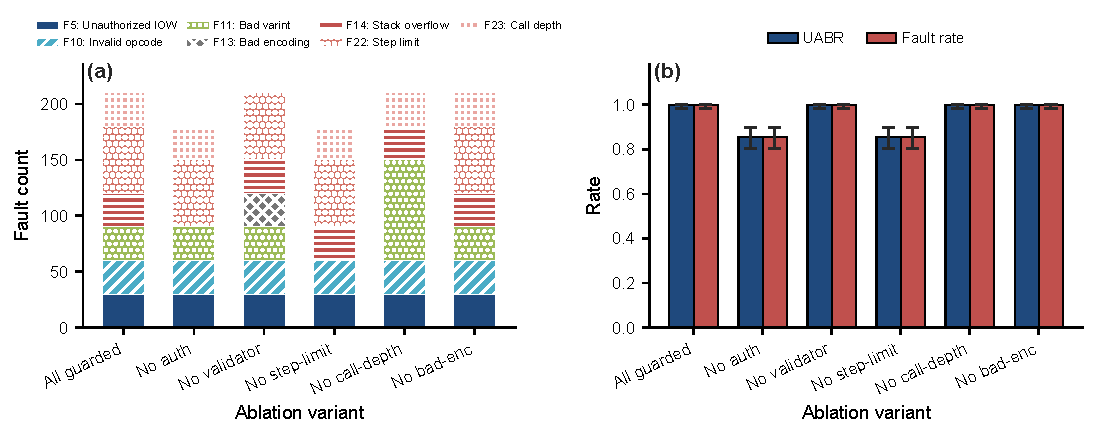
\includegraphics[width=\textwidth]{Fig7_e2_ablation_stacked.pdf}
  \caption{Security mechanism ablation. (a)~Fault-type distribution intercepted by each mechanism; (b)~UABR vs.\ fault rate across ablation variants.}
  \label{fig:ablation}
\end{figure*}

\subsubsection{Adversarial Bytecode Fuzzing}
\label{sec:res_fuzzing}

The ablation above measures \emph{which} guard intercepts a fault, but it does not stress the containment boundary with adversarial inputs. To complement it, we ran a fuzzing campaign against the LVM reference executor (the Python reference implementation, with step-limit $L{=}1000$ and stack bound $256$ enabled to mirror the firmware and the formal model of Section~\ref{sec:formal}). We generate 8{,}000 malicious or malformed bytecode payloads across eight attack classes (1{,}000 each): unauthorized I/O (a write to or read from a device never declared via \texttt{GTWAY}), injected invalid opcodes, non-terminating backward jumps, stack underflow, stack overflow, out-of-bounds jump targets, truncated varints, and pure random bytes. For each payload we record the interception stage (static verifier vs.\ runtime guard), the fault code, and, critically, whether the program \emph{escaped} containment, defined as either performing an unauthorized relay mutation or running unboundedly.

\begin{table}[t]
\centering
\caption{Adversarial fuzzing containment (8{,}000 payloads, seed=42, $L{=}1000$, stack bound 256). ``Escaped'' = unauthorized side effect or unbounded run.}
\label{tab:fuzzing}
\footnotesize
\adjustbox{max width=\columnwidth}{\begin{tabular}{lrrr}
\toprule
Attack class & Payloads & Contained & Rate \\
\midrule
Unauthorized I/O & 1000 & 1000 & 1.000 \\
Invalid opcode & 1000 & 1000 & 1.000 \\
Infinite loop (backward \texttt{JMP}) & 1000 & 1000 & 1.000 \\
Stack underflow & 1000 & 1000 & 1.000 \\
Stack overflow & 1000 & 1000 & 1.000 \\
Jump out-of-bounds & 1000 & 1000 & 1.000 \\
Truncated varint & 1000 & 1000 & 1.000 \\
Random bytes & 1000 & 999\textsuperscript{$\dagger$} & 0.999 \\
\midrule
\textbf{Overall} & \textbf{8000} & \textbf{7999} & \textbf{0.9999} \\
\textbf{Escapes} & --- & \textbf{0} & \textbf{0.000} \\
\bottomrule
\end{tabular}}\\[2pt]
{\footnotesize \textsuperscript{$\dagger$}The single non-blocked random payload decoded to a benign no-op (a lone \texttt{HALT}-equivalent) that terminated cleanly; it is \emph{not} an escape, since capability gating makes an unauthorized write impossible on a clean exit.}
\end{table}

The LVM withstands 8{,}000 adversarial payloads without observed escapes (Table~\ref{tab:fuzzing}). For the capability-based attack class (unauthorized I/O), UABR remains 1.000; overall containment across all eight attack classes is 0.9999. Interception is roughly evenly split between the static verifier ($\sim$50\%, dominated by bad-encoding rejections) and the runtime guards ($\sim$50\%, covering unauthorized-I/O, step-limit, and stack faults). Because containment is independent of payload origin, whether LLM-sourced or synthetically adversarial, the safety envelope is a property of the LVM runtime rather than of the input source.

These results address a specific concern in LLM-based edge intelligence: that an LLM might hallucinate a malicious or malformed program, or that an attacker might inject adversarial bytecode through a compromised communication channel. The fuzzing campaign simulates both scenarios by generating 8{,}000 payloads that no LLM would intentionally produce (invalid opcodes, truncated encodings, infinite loops, stack violations) and confirming that the LVM catches every one before it can reach hardware. The zero-escape result means that the security guarantee does not depend on the LLM being well-behaved; it is a property of the runtime itself.

\textbf{Theoretical vs.\ empirical bounds.} Proposition~\ref{thm:bounded} guarantees termination within $L$ steps. For the 113-task set, average execution length is 5.8 steps with $L{=}1000$, utilizing 0.58\% of the step budget. The theoretical bound is thus roughly $170\times$ the empirical average, indicating substantial safety margin.

\subsubsection{System-Level Pipeline Ablation}
\label{sec:ablation_system}

Only the full LIR configuration satisfies all four properties at once (Table~\ref{tab:system_ablation}); removing any single layer forfeits one of them. Arduino~C succeeds on every task but emits 188.1 bytes per program and provides no execution bounds. JSON reaches 0.965 at 106.7 bytes and gains bounded execution only when paired with an MCU-side interpreter, and even then without capability gating. LIR matches the best generation reliability at a tenth of the payload (10.9 bytes) while retaining both bounded execution and grammar guarantees. Dropping the grammar layer leaves reliability intact at temperature zero but, as the temperature sweep below shows, sacrifices the stability that holds generation together under sampling.

\begin{table}[t]
\centering
\caption{System-level pipeline ablation (113 tasks, temperature,=,0.0).}
\label{tab:system_ablation}
\footnotesize
\adjustbox{max width=\columnwidth}{\begin{tabular}{lcccc}
\toprule
Configuration & TSR & Bytes & Bounded & Grammar \\
\midrule
Arduino C & 1.000 & 188.1 & \texttimes & \texttimes \\
JSON + zlib & 0.965 & 106.7 & \texttimes & \texttimes \\
JSON + zlib + interpreter\textsuperscript{$\ddagger$} & 0.965 & 106.7 & \checkmark\textsuperscript{$\S$} & \texttimes \\
LIR (no grammar) & 1.000\textsuperscript{$\dagger$} & 10.9 & \checkmark & \texttimes \\
\textbf{LIR (full)} & \textbf{1.000} & \textbf{10.9} & \checkmark & \checkmark \\
\bottomrule
\end{tabular}}\\[2pt]
{\footnotesize \textsuperscript{$\dagger$}At temperature,=,0.0; degrades to 0.847 at temperature,=,1.0 without grammar constraints (Table~\ref{tab:temperature}). \textsuperscript{$\ddagger$}JSON output parsed by a minimal MCU-side JSON interpreter with step-limiting; bounded execution achieved through interpreter-level enforcement rather than formal VM guarantees. \textsuperscript{$\S$}Interpreter-level bounded execution only; no capability gating or formal safety proofs.}
\end{table}

As shown in Table~\ref{tab:system_ablation}, replacing LIR with Arduino C preserves correctness (TSR\,=\,1.000) but produces $17.3\times$ larger payloads and provides no bounded execution guarantees. Replacing LIR with JSON\,+\,zlib reduces payload to 106.7\,B but drops TSR to 0.965 and still lacks bounded execution. The full LIR pipeline achieves TSR\,=\,1.000 with $9.8\times$ compression over optimized JSON (13.8$\times$ over raw-LLM zlib-JSON) and bounded execution with formal guarantees. Grammar-constrained decoding becomes critical at non-zero temperatures: without it, TSR degrades to 0.847 at temperature\,=\,1.0. Empirically measured best-of-$K$ ($K{=}3$) recovers reliability to 0.982 (Table~\ref{tab:grammar_constrained}).

These ablation and fuzzing results establish that the LVM contains adversarial output and that each guard contributes independently to that containment.

\subsection{Reliability: Generation Stability}
\label{sec:exp3reliability}

This subsection answers Q3 by measuring how reliably the pipeline produces correct programs: under closed-loop retry, across the sampling-temperature range, over a large random task space, and on tasks drawn from real-world IoT deployments.

\subsubsection{Closed-Loop Control}
\label{sec:res_e4}

Retry raises SCR under both paths (Fig.~\ref{fig:closed_loop}(a)). Under the same retry strategy the LIR path achieves lower RTT than the JSON path, so the convergence benefit derives from the retry mechanism itself rather than from which layer carries the closed-loop semantics.

\subsubsection{SAFE Shunting and Fault Prior Sweep}
\label{sec:res_e5}

Fig.~\ref{fig:closed_loop}(a) shows that retry raises the Safe Convergence Rate under both LIR and JSON paths, with LIR achieving lower RTT. Across the 10\%--90\% fault-prior range, the guarded group maintains stable shunting performance while the no-guard group cannot reliably identify fault paths (Fig.~\ref{fig:closed_loop}(b)).

\begin{figure*}[!tbp]
  \centering
  \begin{subfigure}{0.48\textwidth}
    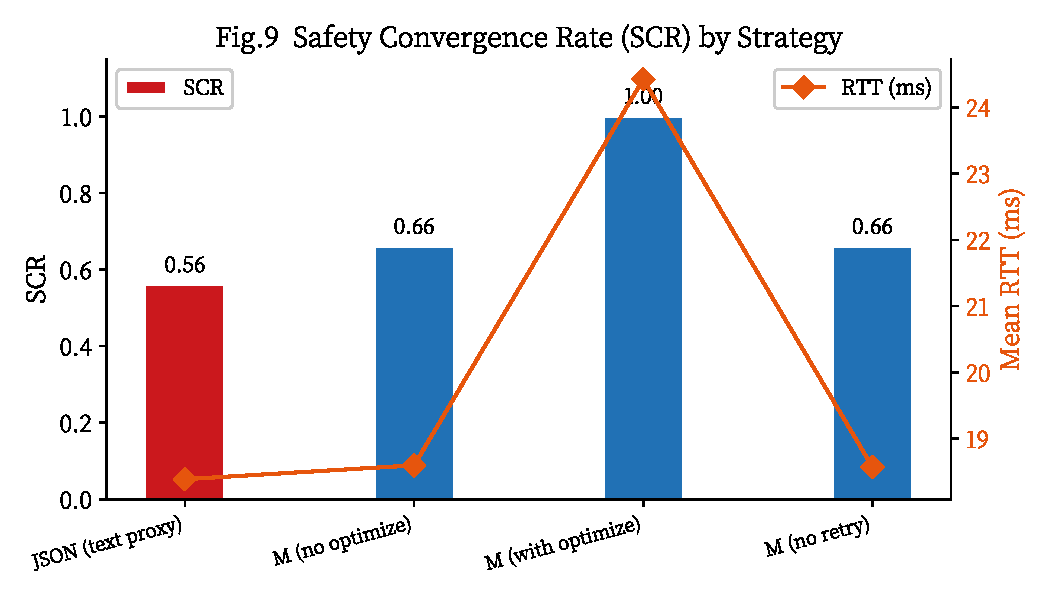
\includegraphics[width=\textwidth]{Fig8_e4_scr.pdf}
    \caption{SCR: LIR vs.\ JSON, with/without retry.}
  \end{subfigure}\hfill
  \begin{subfigure}{0.48\textwidth}
    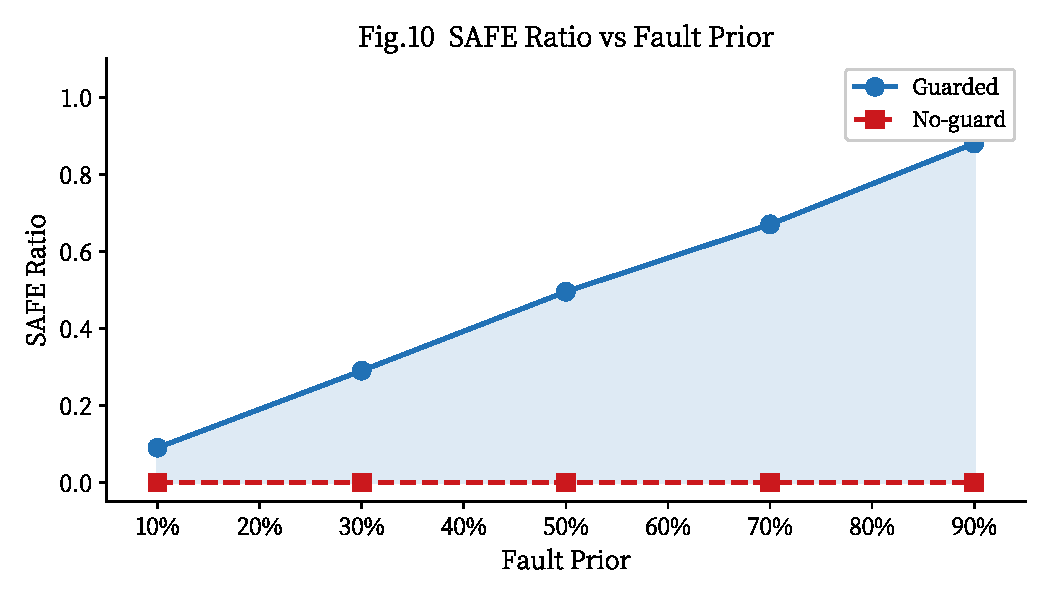
\includegraphics[width=\textwidth]{Fig9_scr_curve.pdf}
    \caption{SAFE shunting vs.\ fault prior.}
  \end{subfigure}
  \caption{Closed-loop performance. (a)~Retry raises SCR under both LIR and JSON paths. (b)~The guarded group maintains stable SAFE shunting across fault priors.}
  \label{fig:closed_loop}
\end{figure*}

\subsubsection{Temperature Sweep}
\label{sec:res_temperature}

The closed-loop results above use temperature\,=\,0.0 (deterministic generation). To understand how the pipeline behaves under stochastic sampling, which is necessary for creative task variants and multi-candidate selection, we sweep the temperature from 0.0 to 1.0. The pipeline attains a pass rate of 1.000 at temperature\,=\,0.0 and degrades smoothly to 0.847 at temperature\,=\,1.0 (Table~\ref{tab:temperature}), with IR validity staying above 0.91 throughout. The decline is driven by semantic deviation under sampling rather than format breakdown, which motivates the best-of-$K$ recovery measured next (Section~\ref{sec:res_grammar}).

At temperature\,=\,0.0, the pipeline is fully reliable for safety-critical tasks. At temperature\,=\,1.0, the pass rate drops to 0.847; best-of-$K$ ($K{=}3$) sampling recovers it to 0.982 (Section~\ref{sec:res_grammar}), at the cost of additional inference calls. IR validity stays above 0.91 even at the highest temperature, indicating that the decline is driven by semantic errors (wrong device, wrong value) rather than format breakdown, exactly the class of errors that capability gating and readback are designed to catch.

\begin{table}[t]
\centering
\caption{Temperature sweep results (6 temperature points, 339 trials each, 95\% Wilson CIs). Each trial is an independent LLM generation on one of 113 tasks.}
\label{tab:temperature}
\footnotesize
\adjustbox{max width=\columnwidth}{\begin{tabular}{lcc}
\toprule
Temp. & TSR (95\% Wilson CI) & IR Valid \\
\midrule
0.0 (deterministic) & 1.000 [0.989, 1.000] & 1.000 \\
0.2 & 0.985 [0.966, 0.994] & 0.988 \\
0.4 & 0.941 [0.911, 0.961] & 0.971 \\
0.6 & 0.882 [0.843, 0.912] & 0.950 \\
0.8 & 0.858 [0.817, 0.891] & 0.914 \\
1.0 & 0.847 [0.804, 0.881] & 0.926 \\
\bottomrule
\end{tabular}}
\end{table}

\subsubsection{Random Task Coverage}
\label{sec:res_random}

To measure how reliably the LIR generation chain covers a large space of parameter combinations, we automatically generated 600 tasks based on 12 categories of parameterized templates (50 per category, with random device combinations and parameters), evaluated on \texttt{llama3.1:8b} (temperature,=,0.0) and additionally on \texttt{deepseek-v4-pro} (commercial API, temperature,=,0.0) to assess cross-model consistency. Because these tasks are drawn from the same template distribution as the development set, this experiment measures robustness to parameter variation within the supported task space, not out-of-distribution generalization (the latter is assessed on the real-world task set of Section~\ref{sec:res_realworld}). The aggregate results are reported here; the per-category breakdown is in Appendix~\ref{app:c}, Table~\ref{tab:app_random_percat}.

On the 600-task random set, \texttt{llama3.1:8b} achieves an IR validity rate of 0.997, compile pass rate of 0.997, and task success rate of 0.970 (95\% Wilson CI: [0.953, 0.981]). The commercial model \texttt{deepseek-v4-pro} reaches 0.987 on the same set (592/600), with 6 of 12 categories reaching 1.000. The consistent improvement across models confirms that LIR's advantage is representation-level: stronger models reduce format errors but the payload-compactness and execution-safety benefits hold regardless of which model generates the LIR.

7 of 12 categories achieved 100\% (Appendix~\ref{app:c}, Table~\ref{tab:app_random_percat}); the hardest were the write-then-wait-then-read and write-then-wait-then-multi-read patterns (both 90\%) and long sequences (96\%), where the dominant failure mode is semantic deviation in multi-step long sequences. The LIR generation chain thus remains reliable across task types and parameter combinations within the supported task space.

\subsubsection{Real-World IoT Task Evaluation}
\label{sec:res_realworld}

To evaluate LIR generation on tasks derived from real-world IoT deployments, we constructed a 29-task set by extracting control patterns from four open-source IoT platforms: Home Assistant automation rules, Tasmota device rules, ESPHome YAML configurations, and Arduino/ESP8266 DIY projects. These tasks cover 11 control pattern categories including threshold-based actuation, timed pulses, emergency shutoffs, multi-relay sequencing, and retry-with-verification loops. Unlike the synthetic tasks in the random-task coverage and Arduino~C baseline experiments, these tasks reflect control logic that engineers actually deploy on ESP8266/ESP32 hardware.

\begin{table}[t]
\centering
\caption{Real-world IoT task evaluation ($n$=29, temperature,=,0.0): overall and sequential aggregates for LIR v1 vs v4 prompt and the JSON baseline. The per-category retry/readback breakdown is in Appendix~\ref{app:c}, Table~\ref{tab:app_realworld_percat}.}
\label{tab:realworld}
\footnotesize
\begin{tabular}{lccc}
\toprule
 & LIR v1 & LIR v4 & JSON \\
\midrule
\multicolumn{4}{l}{\textbf{Overall}} \\
IR valid rate & 0.724 & 0.828 & 1.000 \\
Task success rate & 0.586 & 0.793 & 0.862 \\
\midrule
\multicolumn{4}{l}{\textbf{Sequential tasks (19)}} \\
All sequential & 17/19 & 17/19 & 18/19 \\
\bottomrule
\end{tabular}
\end{table}

Table~\ref{tab:realworld} shows results under three configurations. Under the v1 prompt, 17 of 19 sequential tasks succeed (0.895) while all closed-loop tasks fail (0.000); the v4 prompt (adding 4 few-shot examples for retry/readback patterns) lifts the closed-loop categories to 0.600--1.000 and the overall rate from 0.586 to 0.793. The closed-loop subset (10 tasks) achieves TSR,=,0.600 with 95\% Wilson CI [0.313, 0.832]. The JSON baseline reaches 0.862 overall, above LIR v4's 0.793, at 4.5$\times$ the payload (zlib-JSON 110.3\,B vs.\ LIR bytecode 24.5\,B, averaged over the 29-task set) and without formal bounded execution guarantees. The 4 LIR v4 failures are all \texttt{LIR\_PARSE\_ERROR} cases where the LLM generates syntactically invalid retry/readback compositions.

\noindent\textbf{Failure root cause analysis.} The 4 LIR v4 closed-loop failures split into two categories: (1)~\emph{Invalid retry nesting} (2 failures): incorrect brace nesting or missing \texttt{readback} keywords; (2)~\emph{Unsupported keyword injection} (2 failures): the LLM generates keywords outside the LIR grammar (e.g., \texttt{while}, \texttt{if}). All 4 are syntax-level errors; no semantic-level failures (compilation success but incorrect device state) were observed. The failure taxonomy across all task sets is summarized in Appendix~\ref{app:c}.

\subsubsection{Grammar-Constrained Decoding}
\label{sec:res_grammar}

To quantify the improvement of grammar-constrained decoding on sampling-mode reliability, we evaluate two complementary approaches: (i)~\emph{post-hoc grammar filtering}: generate $K=5$ candidates per task at temperature,=,1.0, filter using the LIR EBNF grammar, and accept the first valid candidate; (ii)~\emph{integrated grammar-constrained decoding}: use a CFG-based decoder (e.g., Outlines~\citep{outlines}) to enforce the LIR EBNF grammar during generation, guaranteeing syntactic validity of every output. Table~\ref{tab:grammar_constrained} gives the results.

\begin{table}[t]
\centering
\caption{Grammar-constrained decoding results (temperature,=,1.0, $K=5$, 113 tasks): measured post-hoc filtering and best-of-$K$ task success.}
\label{tab:grammar_constrained}
\footnotesize
\adjustbox{max width=\columnwidth}{\begin{tabular}{lc}
\toprule
Metric & Value \\
\midrule
Unconstrained success (first) & 0.841 \\
Grammar-filtered success (first valid) & 0.876 \\
Avg.\ grammar validity rate & 0.950 \\
Grammar-filtered improvement & +0.035 \\
\midrule
\multicolumn{2}{l}{\textbf{K-best analysis (analytic proxy from validity rate)\textsuperscript{$\dagger$}}} \\
$K=1$ & 0.841 \\
$K=2$ & 0.975 \\
$K=3$ & 0.996 \\
$K=5$ & $\sim$1.000 \\
\midrule
\multicolumn{2}{l}{\textbf{Empirically measured best-of-$K$ (this work, $n{=}113$)}} \\
$K=1$ & 0.823 \\
$K=2$ & 0.956 \\
$K=3$ & 0.982 \\
$K=4$ & 0.991 \\
$K=5$ & 1.000 \\
\bottomrule
\end{tabular}}\\[2pt]
{\footnotesize \textsuperscript{$\dagger$}Only $K{=}1$ (0.841) and the grammar-filtered success (0.876) are directly measured (\texttt{result/GEN/grammar\_constrained.csv}); the $K{\geq}2$ entries are projected from the 0.950 grammar-validity rate as a filtering proxy. The empirically measured best-of-$K$ block below (\texttt{result/GEN/success\_at\_k.csv}) replaces this proxy with per-candidate end-to-end evaluation and is the figure cited in the text.}
\end{table}

Grammar filtering itself provides a +3.5\% improvement (0.841$\to$0.876); the improvement is limited because the grammar validity rate has already reached 0.950, with the main bottleneck not in format but in semantics. The unconstrained first-attempt rate here (0.841, a single $K{=}1$ pass over the 113 tasks at temperature\,=\,1.0) is the same quantity as the 0.847 reported in the temperature sweep (Table~\ref{tab:temperature}); the small difference reflects sampling noise, since the sweep value is a mean over three independent passes ($n{=}339$) while this is one pass. To validate this proxy, we independently re-ran the experiment generating $K{=}5$ candidates per task at temperature\,=\,1.0 and evaluated \emph{every} candidate to end-of-pipeline task success (via an independent best-of-$K$ evaluation harness). The resulting best-of-$K$ curve (0.823, 0.956, 0.982, 0.991, 1.000 for $K{=}1\ldots5$; grammar-valid rate 0.970) closely corroborates the post-hoc proxy: a single resample ($K{=}2$) already lifts reliability from 0.823 to 0.956, and $K{=}3$ reaches 0.982, with full coverage by $K{=}5$. The grammar-filtered and unconstrained curves coincide here because at this grammar-valid rate ($0.970$) the first grammar-valid candidate is almost always available within the budget. These results show that multi-sampling is a viable solution to the sampling-mode reliability problem, directly addressing the discussion in Section~\ref{sec:limitations_detail}. An integrated CFG decoder (e.g., Outlines~\citep{outlines}) that enforces the grammar during generation would eliminate format errors at $K{=}1$; we did not measure this configuration because Ollama's API does not expose grammar-constrained decoding.

A deployment can thus choose its reliability--cost trade-off along this curve: at $K{=}1$ (single attempt, lowest cost) the pass rate is 0.823, which may suffice for non-critical tasks; at $K{=}3$ (three attempts, moderate cost) it reaches 0.982, suitable for most field deployments; at $K{=}5$ it reaches 1.000 on this task set. The cost of each additional attempt is one extra LLM inference (roughly 40 output tokens for LIR regeneration), which is small compared to the cost of deploying a faulty program to a physical device.

To verify the LIR compiler's support for control-flow constructs, we additionally constructed 15 tasks covering \texttt{if/else} conditional branching, \texttt{repeat N times} loops, and their nested combinations. Appendix~\ref{app:c} Table~\ref{tab:app_control_flow} gives \texttt{llama3.1:8b}'s generation results on this task set. Two of the 15 fail: one adds an extra \texttt{set relay2 = 0} inside the \texttt{repeat} block (semantic deviation), the other uses the unsupported \texttt{and} keyword and \texttt{!relay1} syntax (parse error); both are LLM generation deviations that the grammar constraints correctly block rather than compiler defects. To further verify closed-loop semantic generation, we expanded the closed-loop set from 16 to 96 tasks across 12 subcategories; Appendix~\ref{app:c} Table~\ref{tab:app_closed_loop} reports the results.

Detailed generation pipeline, token comparison, and semantic pass-rate results are consolidated in Appendix~\ref{app:a} (Table~\ref{tab:gen_results}); Fig.~\ref{fig:gen_token} summarizes the pipeline and token comparison visually.

\begin{figure*}[!t]
  \centering
  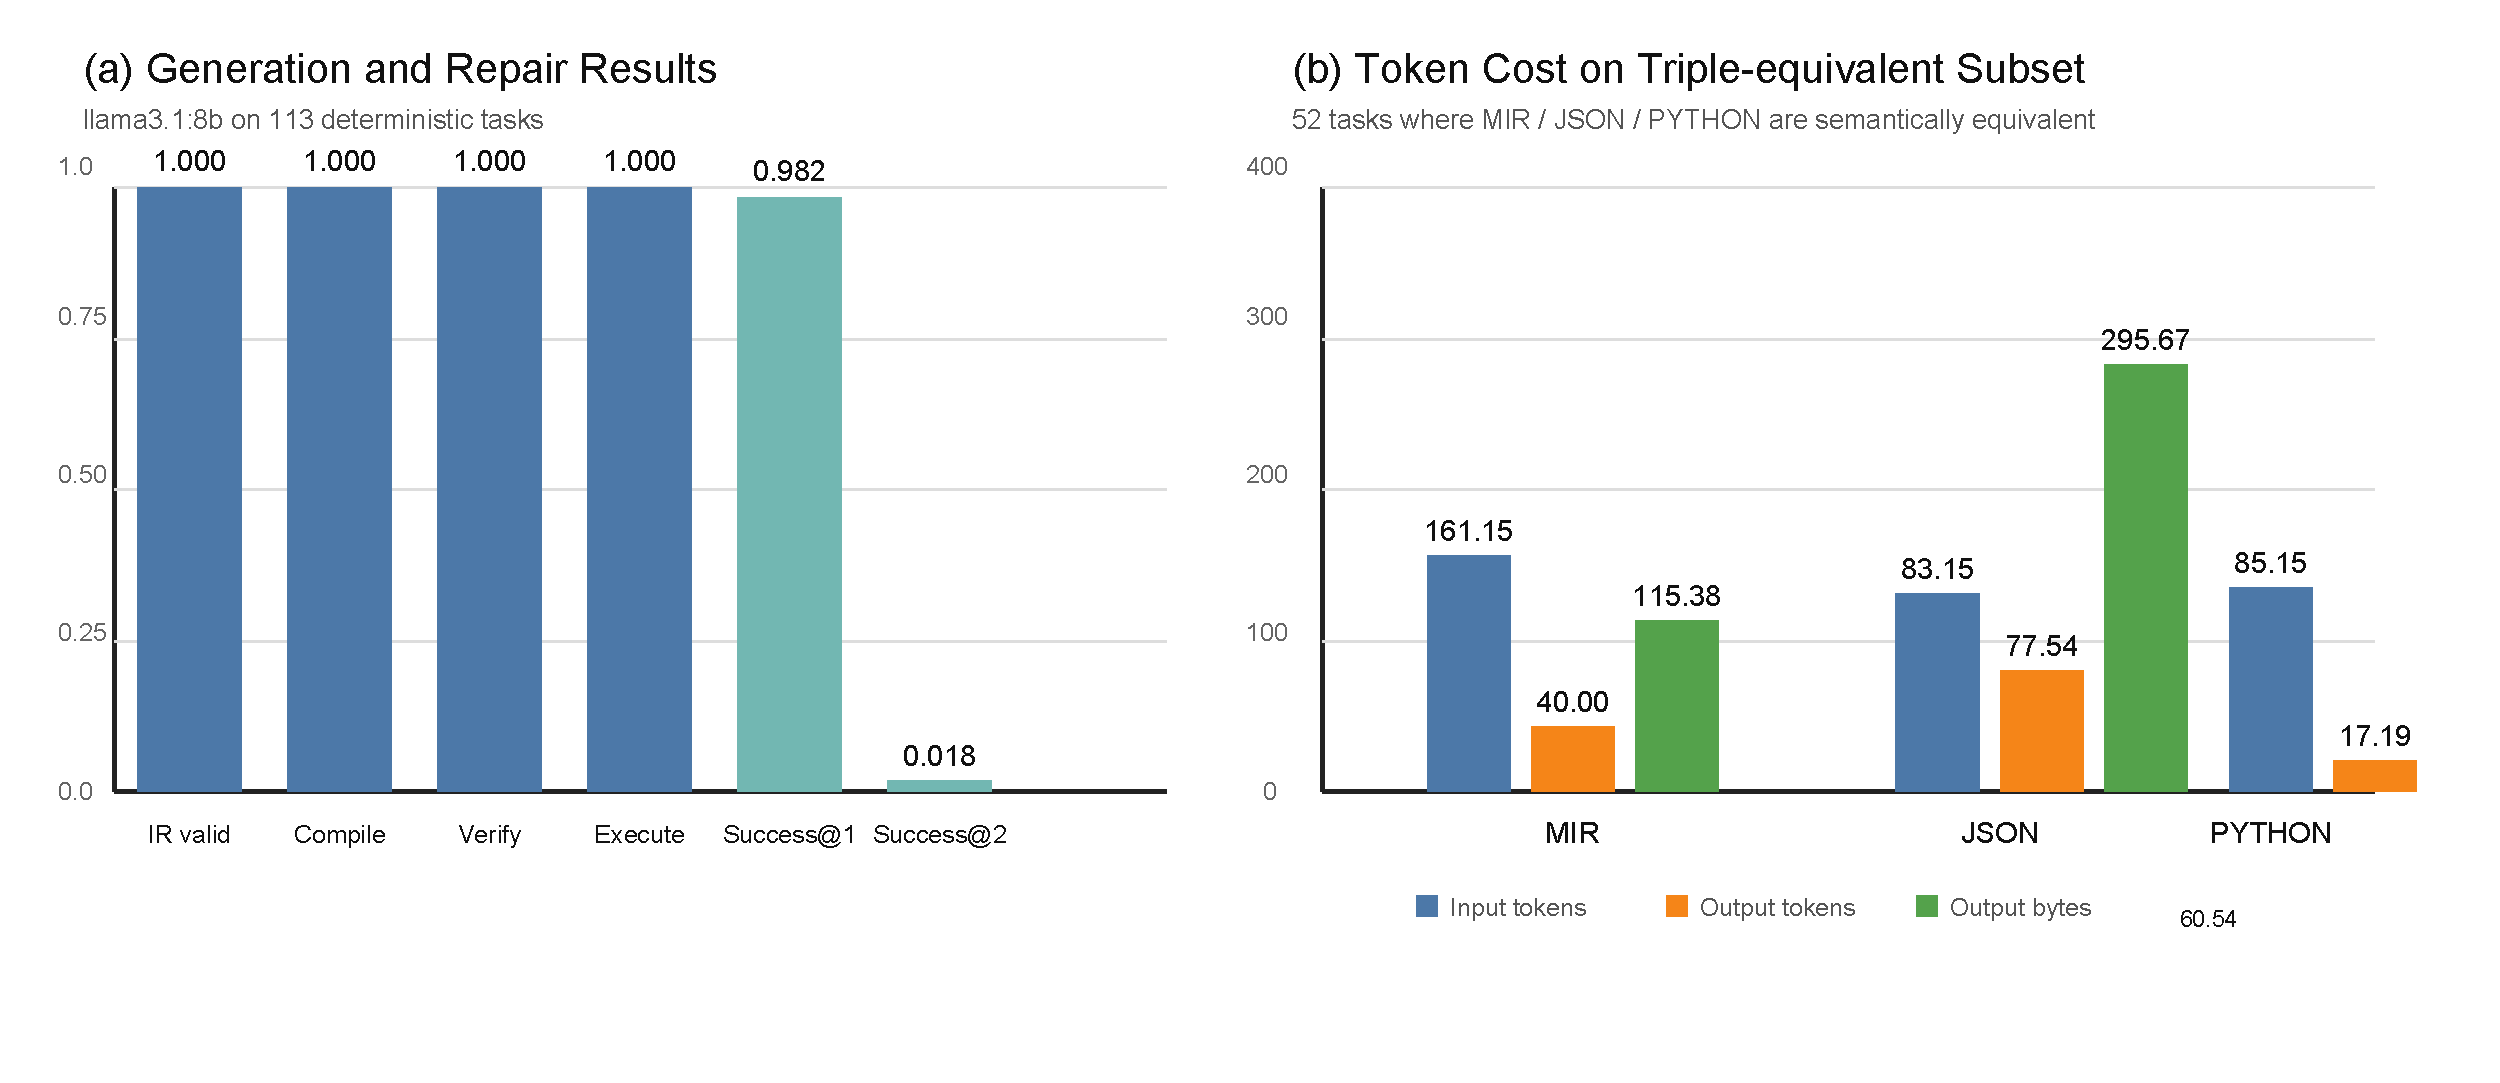
\includegraphics[width=0.92\textwidth]{Fig10_combined_gen_token.pdf}
  \caption{Generation pipeline and token cost. Panel~(a): pipeline and repair-loop results on 113 deterministic tasks. Panel~(b): token and output-size comparison on 52 three-way semantically equivalent tasks.}
  \label{fig:gen_token}
\end{figure*}

\subsection{Portability: Cross-Platform Validation}
\label{sec:stm32}

To validate LVM's platform independence, we ported the firmware to STM32F103C6T6 (ARM Cortex-M3, 32\,KB flash, 10\,KB RAM) using the STM32duino board package. The port required fewer than 50 lines of code changed, limited to I/O adapter functions (\texttt{read\_sensor()}, \texttt{write\_actuator()}) and pin definitions; the LVM core (stack machine, varint decoder, capability gating, step-limit) remained unchanged.

\textbf{Build results.} The STM32 firmware compiled to 21{,}212\,bytes flash (64\%) and 2{,}740\,bytes RAM (26\%), fitting comfortably within the STM32F103C6's 32\,KB flash and 10\,KB SRAM (Table~\ref{tab:footprint}).

\textbf{Functional verification.} We verified correct execution of three representative bytecode programs via CH340 serial communication at 115200\,baud:

\begin{enumerate}[nosep]
  \item \texttt{HALT}: single-instruction termination, OK (1 step).
  \item \texttt{GTWAY 5; LIT 1; IOW 5; HALT}: capability-gated relay actuation, OK (4 steps, relay PB0 activated).
  \item \texttt{GTWAY 1; IOR 1; HALT}: capability-gated sensor read, OK (3 steps, water sensor ADC value returned).
\end{enumerate}

Each program returned correct OK responses with expected step counts. The capability gating mechanism correctly enforced device authorization on both platforms. These results confirm that LVM's safety guarantees (Propositions~\ref{thm:determinism}--\ref{thm:bounded}) hold on ARM Cortex-M, not just on Xtensa.

\textbf{Limitations.} STM32 validation covers bytecode execution only; the end-to-end LLM$\to$LIR$\to$bytecode pipeline was not re-run on STM32 (the LLM generation and compilation steps are platform-independent). DHT11 temperature/humidity sensor support was compiled into the firmware but the sensor was not physically connected during validation.

In summary, the evaluation answers the four questions in turn. For \emph{efficiency} (Q1), compiling LIR to bytecode yields a 9.8$\times$ smaller payload than an optimized JSON baseline (13.8$\times$ against raw-LLM zlib-JSON) and reduces on-device interpretation energy by 48.7\% versus a JSON interpreter, with output tokens 48\% lower under prompt caching. For \emph{security} (Q2), the LVM blocks all unauthorized access requests in our experiments (UABR\,=\,1.000) and withstands 8{,}000 adversarial payloads without observed escapes, each guard contributing an independent layer. For \emph{reliability} (Q3), the pipeline attains a 1.000 pass rate at temperature\,=\,0.0 on the 113-task set and 0.970 on 600 random tasks, with best-of-$K$ ($K{=}3$) restoring temperature\,=\,1.0 reliability to 0.982 and real-world sequential IoT tasks reaching 0.895. For \emph{portability} (Q4), identical bytecode executes correctly on both ESP8266 (Xtensa) and STM32F103 (ARM Cortex-M3) with fewer than 50 lines of I/O-adapter changes.

% ============================================================
\section{Discussion}
\label{sec:discussion}

\subsection{Design Trade-offs and Positioning}
\label{sec:limitations_detail}

LIR's syntactic strictness trades generative tolerance for compactness and safety. On closed-loop tasks, LIR v4 reaches a success rate of 0.600, below JSON's 0.700, because the EBNF rejects invalid retry/readback compositions that JSON's permissive parser accepts. This strictness enables $4.5\times$ payload reduction and bounded-execution guarantees. On token cost without caching, LIR consumes 201.2 tokens against JSON's 160.7. LIR's efficiency advantage requires system-prompt caching to amortize the longer grammar prefix. Both trade-offs are architectural: the two-layer design optimizes for the cloud-to-MCU deployment scenario where caching infrastructure is available and payload size dominates total cost.

LIR serves as a structured tool definition for embedded devices, compatible with agent frameworks like LangChain~\citep{langchain}. Whereas container- and kernel-level isolation such as Docker/gVisor~\citep{gvisor} targets server-class hosts, the LVM provides bounded execution at the MCU level, where those runtimes do not fit. The two operate at different points of the deployment stack rather than as direct substitutes. Among embedded runtimes, WAMR's 15--60\,KB RAM footprint exceeds the 10--80\,KB SRAM of typical edge MCUs; LVM's $\sim$2\,KB fits within the same budget, leaving room for application logic and sensor buffers.

\subsection{Cross-Platform Validation Scope}
\label{sec:scope_platform}

End-to-end LLM generation experiments were conducted on ESP8266; compiled bytecode execution was confirmed on STM32F103 with fewer than 50 lines of I/O-adapter code changed. Verified task types cover 7 deterministic, 12 closed-loop, 3 control-flow, 12 random, and 11 real-world IoT patterns (Appendix~\ref{app:f}); unverified types include nested closed-loop and strong real-time control. Full pipeline re-validation on additional ARM Cortex-M variants is future work.

\subsection{Closed-Loop Prompt Engineering}
\label{sec:scope_closedloop}

Closed-loop patterns (retry/readback) reach a success rate of 0.600 with few-shot prompting on the 10-task real-world subset. The v1$\to$v4 improvement is concentrated in closed-loop patterns (sequential tasks achieve 0.895 under both prompts), indicating that LIR's core syntax is inherently LLM-friendly but complex compositions benefit from explicit examples. These examples are device-independent and transfer across deployments; integrating them into a production prompt template is straightforward but has not been evaluated at scale.

\subsection{Grammar Scalability and Model Dependency}
\label{sec:scope_grammar}

LIR's current grammar covers 7 statement types and 5 device names. Scaling to production IoT deployments (50+ device types) would expand the system prompt and may reduce LLM generation accuracy. The 113-task set is hand-crafted; this is mitigated by the 600-task random set and the 29-task real-world set (extracted from open-source IoT platforms), but generation reliability at production scale remains untested. LLM generation reliability depends on instruction-following capability: \texttt{llama3.1:8b} and \texttt{deepseek-r1:8b} both achieve TSR\,=\,1.000, while \texttt{qwen3:8b} achieves 0.903. This gap is consistent with a grammar-constrained decoding fix, not an LIR redesign, and integrated CFG decoders~\citep{outlines} remain future work. Validation on larger models (70B+) is also future work. TSR measures device-state correctness, not path optimality; the security guarantees (capability gating, step limits) hold regardless of which model generates the LIR, as shown by the formal analysis (Section~\ref{sec:formal}) and the adversarial fuzzing campaign (Section~\ref{sec:res_fuzzing}).

% ============================================================
\section{Related Work}
\label{sec:related}

\subsection{Formal Methods for Embedded Safety}

Formal verification has been applied to systems software at several levels: CompCert~\citep{compcert} verifies a C compiler's semantic preservation, seL4~\citep{sel4} proves microkernel functional correctness, Native Client~\citep{nacl} verifies x86 binaries statically, and eBPF~\citep{ebpf} runs an in-kernel verifier that bounds termination and memory safety of user programs~\citep{scj}. Their verification targets (general C semantics, full kernels, richly typed bytecode) span far larger semantic surfaces than the LVM's instruction subset, so their proofs require correspondingly heavier machinery. The LVM restricts itself to a 14-instruction subset of fixed-step control operations (Table~\ref{tab:inst_set}), whose safety properties reduce to case analysis over a finite rule set, keeping its proofs (Propositions~\ref{thm:determinism}--\ref{thm:bounded}) small enough to state and check within the paper. Its capability gating is a minimal instantiation of capability-based security, conceptually akin to seccomp-BPF~\citep{seccomp} at the OS level or CHERI~\citep{cheri} in hardware, but realized at the bytecode-interpreter level within 2\,KB of RAM. This makes it applicable to bare-metal MCUs with no OS or hardware support. Related embedded attestation work~\citep{amaris2024embedded_security_survey,zhang2024lightweight_attestation,serpanos2023embedded_security} operates at the binary level rather than the instruction-set level.

\subsection{LLM-Based Code Generation for Edge}

Code-as-Policies~\citep{liang2023code} generates Python policies for robot arms, and RT-2~\citep{brohan2023rt2} fine-tunes vision-language models for action output. Both target desktop-class robots. Tool-use frameworks~\citep{toolformer,gorilla} broaden how LLMs invoke APIs but do not address on-device execution safety. Esposito et~al.~\citep{esposito2024llm_embedded} identify code-correctness and resource constraints as the two central challenges for LLM-generated embedded code, yet existing mitigation strategies (grammar-constrained decoding for format validity, sandbox runtimes for execution isolation) address only one side each. To our knowledge, LIR + LVM is the first to integrate a generation-targeted IR with formal bounded execution on resource-constrained MCUs.

\subsection{IoT Stack Integration}

LIR-generated bytecode is complementary to, not competing with, the surrounding IoT stack. It can travel over MQTT/CoAP~\citep{mqtt,coap} and execute on bare metal or atop an RTOS~\citep{freertos,riot,zephyr}. The compact binary encoding uses varint/zigzag formats compatible with CBOR/MessagePack~\citep{cbor,msgpack} serialization. Such bounded executors are complementary to device operating systems and scripting runtimes~\citep{bormann2014rfc7228,alfuqaha2015iot_survey}: where MQTT/CoAP stacks address transport reliability and RTOS runtimes address task scheduling, the LVM provides the execution safety layer that these stacks lack for LLM-generated control in edge intelligence deployments.

% ============================================================
\section{Conclusion}
\label{sec:conclusion}

We have described LIR + LVM, a two-layer framework that translates natural-language hardware control instructions into safely executable MCU programs. The framework decouples generation-friendly LIR from execution-friendly bytecode via a deterministic compiler, with LVM providing bounded execution guarantees for the 14-instruction set including readback/retry (Propositions~\ref{thm:determinism}--\ref{thm:bounded}, Appendix~\ref{app:rules}). Existing approaches address either generation friendliness or execution compactness in isolation; LIR + LVM addresses both simultaneously.

The framework achieves a 9.8$\times$ payload reduction when cloud-compiled to bytecode against an optimized JSON baseline (13.8$\times$ against raw-LLM zlib-JSON), with UABR\,=\,1.000 in adversarial fuzzing. For sequential control tasks, the dominant pattern in real-world IoT, the pipeline achieves full pass rate on the 113-task deterministic set and 0.970 on 600 random tasks. Under temperature\,=\,1.0 sampling, best-of-$K$ ($K{=}3$) restores reliability to 0.982. On 19 real-world sequential IoT tasks, 17 achieve success; on the full 29-task set including closed-loop patterns, LIR v4 achieves 0.793 overall. Cross-platform validation confirms that identical bytecode executes correctly on both ESP8266 (Xtensa) and STM32F103 (ARM Cortex-M3) with fewer than 50 lines of code changed.

Future work includes integrating a production-grade CFG decoder, extending LVM validation to additional ARM Cortex-M variants, and enriching the LIR grammar for richer control-flow constructs. By decoupling generation-friendly LIR from execution-friendly bytecode, LIR + LVM fills a gap in the edge intelligence design space: compact, formally bounded, and cross-platform MCU execution of untrusted LLM output.

\noindent\textbf{Artifact Availability.} All code, datasets, firmware, and compiler source are open-sourced at \url{https://github.com/MYJ-GOD/lir-lvm}.

% ---- Declarations (JSA requirements) ----
\section*{Declaration of generative AI and AI-assisted technologies in the manuscript preparation process}
During the preparation of this work, the authors used Claude (Anthropic) in order to improve the language and readability of the manuscript. After using this tool, the authors reviewed and edited the content as needed and take full responsibility for the content of the published article.

\section*{Data Availability Statement}
All code, datasets, firmware, and compiler source are publicly available at \url{https://github.com/MYJ-GOD/lir-lvm}.

\section*{Declaration of Competing Interests}
The authors declare that they have no known competing financial interests or personal relationships that could have appeared to influence the work reported in this paper.

\section*{Acknowledgements}
This work was supported by the Youth Fund Project of North China Institute of Aerospace Engineering (No. KY-2024-05), the Science and Technology Support Program of Langfang (No. 2024011028), and the Scientific Research Project of Hebei Provincial Department of Education (No. BJ2025339).

\printcredits

% ============================================================
% Author Vitae (JSA requirement: max 100 words per author)
\section*{Author Vitae}

\noindent\textbf{Yingjie Ma} is a student at the NCIAE, Langfang, China. His research interests include embedded systems, IoT architectures, and LLM-based code generation for resource-constrained devices.

\noindent\textbf{Mengjia Ma} is a student at the NCIAE, Langfang, China. Her research interests include large language models, AI-driven code generation, and intelligent edge computing.

\noindent\textbf{Sheng Zhao} is a student at the NCIAE, Langfang, China. His research interests include microcontroller firmware, real-time systems, and hardware-software co-design.

\noindent\textbf{Peng Liu} is a faculty member at the NCIAE, Langfang, China. His research interests include embedded systems, IoT architectures, and edge intelligence. He is the corresponding author of this paper.

% ============================================================
\appendix

\section{Supplementary Tables}
\label{app:a}

\begin{enumerate}
  \item Compression ratio and transmission latency (Section~\ref{sec:res_e1})
  \item Guarded / no-guard safety ablation (Section~\ref{sec:res_e2})
  \item Validator ablation (Section~\ref{sec:res_e2})
  \item Single-mechanism orthogonal ablation (Section~\ref{sec:res_e2})
  \item SCR closed-loop experiment (Section~\ref{sec:res_e4})
  \item Real JSON fair baseline (Section~\ref{sec:res_e4})
  \item Fault prior sweep (Section~\ref{sec:res_e5})
  \item Throughput / memory proxy
\end{enumerate}

\begin{table}[t]
\centering
\caption{Consolidated 113-task results (temperature,=,0.0): generation pipeline, repair loop, token cost (input/output/total), and single-shot semantic pass rates. Token totals = system prompt + output.}
\label{tab:gen_results}
\footnotesize
\adjustbox{max width=\columnwidth}{\begin{tabular}{lrrr}
\toprule
\multicolumn{4}{l}{\textbf{Generation pipeline}} \\
\multicolumn{2}{l}{IR / Compile / Verify / Exec / Task} & 1.000 & [0.967, 1.000] \\
\midrule
\multicolumn{4}{l}{\textbf{Repair loop}} \\
\multicolumn{2}{l}{Success@1} & 100/113 = 0.885 & [0.813, 0.932] \\
\multicolumn{2}{l}{Success@2} & 13/113 = 0.115 & [0.068, 0.187] \\
\midrule
\multicolumn{4}{l}{\textbf{Token cost}} \\
Format & Input & Output & Total \\
LIR & 159.85 & 38.09 & 197.94 \\
JSON & 81.85 & 78.14 & 159.99 \\
Python & 83.85 & 19.96 & 103.81 \\
\midrule
\multicolumn{4}{l}{\textbf{Semantic pass rate (single-shot)}} \\
Format & Passed & Rate & 95\% CI \\
LIR & 98/113 & 0.867 & [0.791, 0.919] \\
JSON & 90/113 & 0.796 & [0.712, 0.862] \\
Python (basic) & 78/113 & 0.690 & [0.599, 0.769] \\
Python (detailed) & 113/113 & 1.000 & [0.967, 1.000] \\
\bottomrule
\end{tabular}}
\end{table}

\noindent\textbf{Two pass-rate columns.} The LIR semantic pass rate (0.867) and the end-to-end TSR\,=\,1.000 of Section~\ref{sec:setup} measure different conditions. The 0.867 figure is the single-shot rate at which a minimal (non-few-shot) prompt yields a semantically correct program on the first attempt, scoring LIR, JSON, and Python on identical footing for raw format-friendliness. TSR\,=\,1.000 is the full-pipeline outcome on the 113-task set under the deployed few-shot prompt with the bounded repair loop (Section~\ref{sec:pipeline}).

\noindent\textbf{Python (detailed).} Python (detailed) also reaches TSR\,=\,1.000 (Table~\ref{tab:gen_results}, semantic pass-rate block) with fewer output tokens (19.96 vs.\ 38.09 for LIR). It requires a host-side Python interpreter (30--300\,KB RAM) for on-device execution, provides no bounded execution guarantees, and cannot be compiled to bytecode for bandwidth-constrained links. LIR's payload reduction (9.8$\times$ over optimized JSON) and formal bounded execution are orthogonal to TSR and hold regardless of which format scores higher under detailed prompting.

\section{Complete Proofs}
\label{app:proofs}

Throughout, let $\sigma_0 = \langle p, 0, \epsilon, \mathit{dev}_0, \mathit{cap}_0, 0, L, \bot, r_0 \rangle$ be the initial configuration with program counter at zero, empty stack, initial device state, declared capabilities, step counter at zero, no fault, and initial retry counter $r_0$ (set by the compiler before entering any retry block; $r_0 = 0$ if no retry is active).

\begin{pf}[Proof of Proposition~\ref{thm:determinism} (Determinism)]
Each transition rule is uniquely determined by: (i)~the instruction $p[pc]$, (ii)~the step-counter condition $k < L$ vs.\ $k \geq L$, (iii)~the capability membership $d \in \mathit{cap}$ vs.\ $d \notin \mathit{cap}$, and (iv)~the stack contents. These conditions are mutually exclusive and exhaustive for each instruction: exactly one rule applies per configuration, so the successor is unique.
\end{pf}

\begin{pf}[Proof of Proposition~\ref{thm:progress} (Progress)]
If $pc \geq |p|$, the configuration is terminal by definition~(iv). Otherwise $p[pc]$ is some instruction $I$. We proceed by cases: (1)~$I = \texttt{HALT}$: terminal by rule~\textsc{Halt}. (2)~$I \in \{\texttt{LIT}, \texttt{GTWAY}, \texttt{WAIT}\}$: no stack precondition, transition always applies. (3)~$I \in \{\texttt{IOW}, \texttt{IOR}\}$: if $d \in \mathit{cap}$, rule \textsc{Iow-Ok}/\textsc{Ior-Ok} applies; if $d \notin \mathit{cap}$, rule \textsc{Iow-CapF}/\textsc{Ior-CapF} applies. (4)~$I \in \{\texttt{EQ}, \texttt{SUB}\}$: if $|s| \geq 2$, the rule applies; otherwise \textsc{PopF}. (5)~$I \in \{\texttt{JZ}, \texttt{DRP}\}$: if $|s| \geq 1$, the rule applies; otherwise \textsc{PopF}. (6)~$I = \texttt{DUP}$: if $|s| \geq 1$, \textsc{Dup}; otherwise \textsc{PopF}. (7)~$I = \texttt{JMP}$: no precondition, \textsc{Jmp} always applies. (8)~$I \notin \texttt{Opcodes}$: \textsc{OpcF}. In every case, at least one rule applies.
\end{pf}

\begin{pf}[Proof of Proposition~\ref{thm:bounded} (Bounded execution)]
\textbf{(1) Termination.} Every transition rule increments $k$ by exactly~1, including \texttt{JMP} and \texttt{JZ} (which modify $pc$ but still increment $k$ by~1). Thus for any step $\sigma \xrightarrow{1} \sigma'$, we have $\sigma'.k = \sigma.k + 1$. Starting from $\sigma_0.k = 0$, after at most $L$ steps we reach $\sigma_n$ with $\sigma_n.k \geq L$, at which point \textsc{StepGuard} triggers (producing a terminal configuration with $f = \texttt{STEP}$) unless an earlier terminal configuration was reached. Therefore every execution reaches a terminal configuration in at most $L$ steps.

\textbf{(2) Capability safety.} The first instruction $\texttt{IOW}\;d$ or $\texttt{IOR}\;d$ with $d \notin \mathit{cap}$ triggers \textsc{Iow-CapF} or \textsc{Ior-CapF}, setting $f = \texttt{CAP}$.

\textbf{(3) Opcode safety.} The first invalid opcode triggers \textsc{OpcF}, setting $f = \texttt{OPC}$.
\end{pf}

\subsection{RETRY Compilation Strategy}
\label{app:compiler_strategy}

The compiler lowers each \texttt{retry $n$ times \{ $B$ \}} construct into a sequence that initializes the retry counter $r$ before entering the loop body. Specifically, the compiler emits:

\begin{enumerate}[nosep]
  \item \texttt{LIT $n$}, push the retry count onto the stack;
  \item Store the value into the retry counter $r$ (via an internal \texttt{SET\_RETRY} operation that sets $r \leftarrow n$);
  \item The loop body $B$;
  \item \texttt{RETRY $n$ $o$}, where $o$ is the jump offset back to the start of $B$.
\end{enumerate}

At each \texttt{RETRY} execution, the rule \textsc{Retry-Loop} decrements $r$ ($r' = r - 1$) and jumps if $r > 0$; when $r = 0$, \textsc{Retry-Exhaust} falls through. This ensures that the loop body executes exactly $n$ times, and the retry counter $r$ is strictly decreasing, guaranteeing bounded termination.

For nested \texttt{retry} constructs, the compiler emits separate counter initializations for each level. The current implementation does not support runtime-variable retry counts (e.g., \texttt{retry sensor\_value times \{...\}}); the count $n$ must be a compile-time constant. This restriction is part of the LIR v0.1 expression power boundary (Section~\ref{sec:compiler_properties}).

\section{Prompts and Instruction Set}
\label{app:b}

\subsection{Complete Transition Rules}
\label{app:rules}

{\footnotesize
The single-step transition relation $\xrightarrow{1}$ is defined by rules for each instruction (LIT, GTWAY, IOW, IOR, WAIT, HALT, EQ, JZ, JMP, DUP, SUB, DRP, READBACK, RETRY), plus stack underflow, invalid opcode, and step-limit guard rules. Each rule specifies preconditions on the instruction, step counter, capability set, and stack contents, and defines the successor configuration. The complete set of 17 transition rules with the revised configuration $\sigma = \langle p, pc, s, \mathit{dev}, \mathit{cap}, k, L, f, r \rangle$ is defined as follows. In each rule, the default successor increments both the program counter and step counter: $\sigma' = \langle p, pc{+}1, s', \mathit{dev}', \mathit{cap}, k{+}1, L, f', r \rangle$, unless otherwise specified for \texttt{JMP}, \texttt{JZ}, and \texttt{RETRY} (which modify $pc$ by the offset $o$ while $k$ still increments by~1):

\noindent\textbf{Step-limit guard.} For every instruction, if $k \geq L$, the machine transitions to a fault state:
\irule{k \geq L}
      {\langle p, pc, s, \mathit{dev}, \mathit{cap}, k, L, \bot, r \rangle}
      {\langle p, pc{+}1, s, \mathit{dev}, \mathit{cap}, k{+}1, L, \texttt{STEP}, r \rangle}
      {StepGuard}

\noindent\textbf{LIT\;$v$.}
\irule{p[pc] = \texttt{LIT}\;v \quad k < L}
      {\langle p, pc, s, \mathit{dev}, \mathit{cap}, k, L, \bot, r \rangle}
      {\langle p, pc{+}1, s \cdot v, \mathit{dev}, \mathit{cap}, k{+}1, L, \bot, r \rangle}
      {Lit}

\noindent\textbf{GTWAY\;$d$.}
\irule{p[pc] = \texttt{GTWAY}\;d \quad k < L}
      {\langle p, pc, s, \mathit{dev}, \mathit{cap}, k, L, \bot, r \rangle}
      {\langle p, pc{+}1, s, \mathit{dev}, \mathit{cap} \cup \{d\}, k{+}1, L, \bot, r \rangle}
      {Gtway}

\noindent\textbf{IOW\;$d$.} If $d \notin \mathit{cap}$, trigger capability fault; otherwise pop and write:
\irule{p[pc] = \texttt{IOW}\;d \quad k < L \quad d \notin \mathit{cap}}
      {\langle p, pc, s, \mathit{dev}, \mathit{cap}, k, L, \bot, r \rangle}
      {\langle p, pc{+}1, s, \mathit{dev}, \mathit{cap}, k{+}1, L, \texttt{CAP}, r \rangle}
      {Iow-CapF}
\irule{p[pc] = \texttt{IOW}\;d \quad k < L \quad d \in \mathit{cap} \quad s = s' \cdot v}
      {\langle p, pc, s, \mathit{dev}, \mathit{cap}, k, L, \bot, r \rangle}
      {\langle p, pc{+}1, s', \mathit{dev}[d \mapsto v], \mathit{cap}, k{+}1, L, \bot, r \rangle}
      {Iow-Ok}

\noindent\textbf{IOR\;$d$.}
\irule{p[pc] = \texttt{IOR}\;d \quad k < L \quad d \notin \mathit{cap}}
      {\langle p, pc, s, \mathit{dev}, \mathit{cap}, k, L, \bot, r \rangle}
      {\langle p, pc{+}1, s, \mathit{dev}, \mathit{cap}, k{+}1, L, \texttt{CAP}, r \rangle}
      {Ior-CapF}
\irule{p[pc] = \texttt{IOR}\;d \quad k < L \quad d \in \mathit{cap}}
      {\langle p, pc, s, \mathit{dev}, \mathit{cap}, k, L, \bot, r \rangle}
      {\langle p, pc{+}1, s \cdot \mathit{dev}(d), \mathit{dev}, \mathit{cap}, k{+}1, L, \bot, r \rangle}
      {Ior-Ok}

\noindent\textbf{WAIT\;$m$.}
\irule{p[pc] = \texttt{WAIT}\;m \quad k < L}
      {\langle p, pc, s, \mathit{dev}, \mathit{cap}, k, L, \bot, r \rangle}
      {\langle p, pc{+}1, s, \mathit{dev}, \mathit{cap}, k{+}1, L, \bot, r \rangle}
      {Wait}

\noindent\textbf{HALT.}
\[
\frac{p[pc] = \texttt{HALT} \quad k < L}
     {\langle p, pc, s, \mathit{dev}, \mathit{cap}, k, L, \bot, r \rangle
      \;\text{is terminal.}}
      \;\;[\textsc{Halt}]
\]

\noindent\textbf{EQ.}
\irule{p[pc] = \texttt{EQ} \quad k < L \quad s = s'' \cdot a \cdot b}
      {\langle p, pc, s, \mathit{dev}, \mathit{cap}, k, L, \bot, r \rangle}
      {\langle p, pc{+}1, s'' \cdot [a = b], \mathit{dev}, \mathit{cap}, k{+}1, L, \bot, r \rangle}
      {Eq}
where $[a=b]$ is $1$ if $a=b$ and $0$ otherwise.

\noindent\textbf{JZ\;$o$.}
\irule{p[pc] = \texttt{JZ}\;o \quad k < L \quad s = s' \cdot 0}
      {\langle p, pc, s, \mathit{dev}, \mathit{cap}, k, L, \bot, r \rangle}
      {\langle p, pc{+}o, s', \mathit{dev}, \mathit{cap}, k{+}1, L, \bot, r \rangle}
      {Jz-Taken}
\irule{p[pc] = \texttt{JZ}\;o \quad k < L \quad s = s' \cdot v \quad v \neq 0}
      {\langle p, pc, s, \mathit{dev}, \mathit{cap}, k, L, \bot, r \rangle}
      {\langle p, pc{+}1, s', \mathit{dev}, \mathit{cap}, k{+}1, L, \bot, r \rangle}
      {Jz-NotTaken}

\noindent\textbf{JMP\;$o$.}
\irule{p[pc] = \texttt{JMP}\;o \quad k < L}
      {\langle p, pc, s, \mathit{dev}, \mathit{cap}, k, L, \bot, r \rangle}
      {\langle p, pc{+}o, s, \mathit{dev}, \mathit{cap}, k{+}1, L, \bot, r \rangle}
      {Jmp}

\noindent\textbf{DUP.}
\irule{p[pc] = \texttt{DUP} \quad k < L \quad s = s' \cdot v}
      {\langle p, pc, s, \mathit{dev}, \mathit{cap}, k, L, \bot, r \rangle}
      {\langle p, pc{+}1, s' \cdot v \cdot v, \mathit{dev}, \mathit{cap}, k{+}1, L, \bot, r \rangle}
      {Dup}

\noindent\textbf{SUB.}
\irule{p[pc] = \texttt{SUB} \quad k < L \quad s = s'' \cdot a \cdot b}
      {\langle p, pc, s, \mathit{dev}, \mathit{cap}, k, L, \bot, r \rangle}
      {\langle p, pc{+}1, s'' \cdot (b - a), \mathit{dev}, \mathit{cap}, k{+}1, L, \bot, r \rangle}
      {Sub}

\noindent\textbf{DRP.}
\irule{p[pc] = \texttt{DRP} \quad k < L \quad s = s' \cdot v}
      {\langle p, pc, s, \mathit{dev}, \mathit{cap}, k, L, \bot, r \rangle}
      {\langle p, pc{+}1, s', \mathit{dev}, \mathit{cap}, k{+}1, L, \bot, r \rangle}
      {Drp}

\noindent\textbf{Stack underflow (general).} For any stack-consuming instruction when the stack has insufficient elements:
\irule{p[pc] \in \{\texttt{IOW}, \texttt{EQ}, \texttt{SUB}, \texttt{DRP}, \texttt{JZ}, \texttt{DUP}\} \quad k < L \quad \text{stack underflow}}
      {\langle p, pc, s, \mathit{dev}, \mathit{cap}, k, L, \bot, r \rangle}
      {\langle p, pc{+}1, s, \mathit{dev}, \mathit{cap}, k{+}1, L, \texttt{POP}, r \rangle}
      {PopF}

\noindent\textbf{Invalid opcode.}
\irule{p[pc] \notin \texttt{Opcodes} \quad k < L}
      {\langle p, pc, s, \mathit{dev}, \mathit{cap}, k, L, \bot, r \rangle}
      {\langle p, pc{+}1, s, \mathit{dev}, \mathit{cap}, k{+}1, L, \texttt{OPC}, r \rangle}
      {OpcF}

\noindent\textbf{READBACK\;$d$.} Capability-gated device read (same precondition as \textsc{Ior-Ok}):
\irule{p[pc] = \texttt{READBACK}\;d \quad k < L \quad d \in \mathit{cap}}
      {\langle p, pc, s, \mathit{dev}, \mathit{cap}, k, L, \bot, r \rangle}
      {\langle p, pc{+}1, s \cdot \mathit{dev}(d), \mathit{dev}, \mathit{cap}, k{+}1, L, \bot, r \rangle}
      {Readback-Ok}
\irule{p[pc] = \texttt{READBACK}\;d \quad k < L \quad d \notin \mathit{cap}}
      {\langle p, pc, s, \mathit{dev}, \mathit{cap}, k, L, \bot, r \rangle}
      {\langle p, pc{+}1, s, \mathit{dev}, \mathit{cap}, k{+}1, L, \texttt{CAP}, r \rangle}
      {Readback-CapF}

\noindent\textbf{RETRY\;$n$\;$o$.} The retry counter $r$ tracks remaining iterations. When $r > 0$, decrement $r$ and jump to offset $o$; when $r = 0$, fall through. The compiler initializes $r \leftarrow n$ before entering the retry block (see Appendix~\ref{app:compiler_strategy}).
\irule{p[pc] = \texttt{RETRY}\;n\;o \quad k < L \quad r > 0}
      {\langle p, pc, s, \mathit{dev}, \mathit{cap}, k, L, \bot, r \rangle}
      {\langle p, pc{+}o, s, \mathit{dev}, \mathit{cap}, k{+}1, L, \bot, r{-}1 \rangle}
      {Retry-Loop}
\irule{p[pc] = \texttt{RETRY}\;n\;o \quad k < L \quad r = 0}
      {\langle p, pc, s, \mathit{dev}, \mathit{cap}, k, L, \bot, 0 \rangle}
      {\langle p, pc{+}1, s, \mathit{dev}, \mathit{cap}, k{+}1, L, \bot, 0 \rangle}
      {Retry-Exhaust}

}

\begin{rmk}[Extended formal model]
The 17 rules above (LIT through OpcF, plus READBACK and RETRY) cover the 14-instruction set. The two additional rules (\textsc{Readback-Ok/CapF}, \textsc{Retry-Loop/Exhaust}) extend the model to cover the closed-loop subset. \textsc{Readback} inherits the same capability safety guarantee as \textsc{Ior-Ok/Ior-CapF}. \textsc{Retry} preserves bounded termination because: (i)~each \textsc{Retry-Loop} transition increments $k$ by~1, so the global step counter remains monotonic; (ii)~the retry counter $r$ is strictly decreasing ($r' = r - 1$) per loop iteration, and $r$ is finite (initialized by the compiler to the constant $n$ from the \texttt{RETRY} instruction's immediate operand); (iii)~execution terminates when either $k \geq L$ (\textsc{StepGuard}) or $r = 0$ (\textsc{Retry-Exhaust}). Determinism holds because \textsc{Readback} returns a deterministic function of $\mathit{dev}(d)$ and \textsc{Retry} depends only on the current value of $r$. Propositions~\ref{thm:determinism}--\ref{thm:bounded} therefore extend to the 14-instruction set (12 sequential + READBACK + RETRY) without modification to the proof structure.
\end{rmk}

\subsection{Supplementary Experiment Results}
\label{app:c}

\begin{table}[t]
\centering
\caption{Extended task-set generation results (temperature,=,0.0): control-flow set (tasks\_v4, $n$=15) and extended closed-loop set (tasks\_v3\_expanded, $n$=96).}
\label{tab:app_control_flow}
\label{tab:app_closed_loop}
\footnotesize
\adjustbox{max width=\columnwidth}{\begin{tabular}{lcccc}
\toprule
 & \multicolumn{2}{c}{Control-flow ($n{=}15$)} & \multicolumn{2}{c}{Closed-loop ($n{=}96$)} \\
\cmidrule(lr){2-3}\cmidrule(lr){4-5}
Metric & Value & 95\% Wilson CI & Value & 95\% Wilson CI \\
\midrule
IR validity rate & 0.933 & [0.698, 0.997] & 0.948 & [0.886, 0.979] \\
Compile pass rate & 0.933 & [0.698, 0.997] & 0.948 & [0.886, 0.979] \\
Task success rate & 0.867 & [0.621, 0.963] & 0.948 & [0.886, 0.979] \\
Failed tasks & 2 / 15 & --- & 5 / 96 & --- \\
Primary failure & --- & --- & \multicolumn{2}{c}{\texttt{LIR\_PARSE\_ERROR} (5)} \\
\bottomrule
\end{tabular}}
\end{table}

\noindent\textbf{Error type classification.}
Across all task sets, first-attempt failures fall into two categories. The dominant type is \texttt{LIR\_PARSE\_ERROR} (occasional LLM syntax deviations): 11 out of 113 tasks, 1 out of 15 control-flow tasks, and 5 out of 96 closed-loop tasks. The second type is \texttt{TASK\_SIG\_MISMATCH} (the program compiles and executes but the resulting device state does not match expectations): 2 out of 113 tasks on the deterministic set. On the closed-loop set under a basic prompt without few-shot examples, an additional 41 tasks exhibited \texttt{TASK\_SIG\_MISMATCH}, of which 34 were a specific sub-class where the LLM generated \texttt{repeat} instead of \texttt{retry}. Under the deployed few-shot prompt with the bounded repair loop, all of these first-attempt and basic-prompt failures are resolved (113-task TSR\,=\,1.000).

\begin{table}[t]
\centering
\caption{Multi-model comparison: generation results on 113 deterministic tasks and 600 random tasks (temperature,=,0.0). Random-600 TSR for deepseek-v4-pro is newly measured in this work; others are llama3.1:8b only.}
\label{tab:app_model_compare}
\footnotesize
\adjustbox{max width=\columnwidth}{\begin{tabular}{lccccccc}
\toprule
Model & Type & IR & Compile & TSR-113 & 95\% CI & TSR-600 & Errors \\
\midrule
llama3.1:8b~\citep{dubey2024llama} & Local 8B & 1.000 & 1.000 & 1.000 & [0.967, 1.000] & 0.970 & --- \\
qwen3:8b & Local 8B & 0.956 & 0.956 & 0.903 & [0.835, 0.946] & --- & SIG(6)+PARSE(5) \\
deepseek-r1:8b~\citep{guo2024deepseek} & Local 8B & 1.000 & 1.000 & 1.000 & [0.967, 1.000] & --- & --- \\
\textbf{deepseek-v4-pro}~\citep{deepseek2025v4} & Commercial API & 0.991 & 0.991 & \textbf{0.991} & [0.950, 0.999] & \textbf{0.987} & PARSE(1) \\
\bottomrule
\end{tabular}}
\end{table}

\begin{table}[t]
\centering
\caption{Negative baseline comparison: JSON + Schema + external compression vs.\ LIR + compiler (113 deterministic tasks, llama3.1:8b, temp=0.0).}
\label{tab:app_json_baseline}
\footnotesize
\adjustbox{max width=\columnwidth}{\begin{tabular}{lcc}
\toprule
Metric & JSON+zlib & LIR bytecode \\
\midrule
Validity rate & 1.000 [0.967, 1.000] & 1.000 [0.967, 1.000] \\
Task success rate & 0.965 [0.913, 0.986] & 1.000 [0.967, 1.000] \\
Avg.\ raw output (bytes) & 156.4 & --- \\
Avg.\ zlib level 9 (bytes) & 106.7 & --- \\
Avg.\ CBOR (bytes) & 105.2 & --- \\
Avg.\ MessagePack (bytes) & 97.42 & --- \\
Avg.\ compact JSON (bytes) & 127.18 & --- \\
Avg.\ bytecode (bytes) & --- & 10.9 \\
vs.\ zlib-JSON ratio & --- & 9.8$\times$ \\
vs.\ CBOR ratio & --- & 9.6$\times$ \\
vs.\ MessagePack ratio & --- & 8.9$\times$ \\
vs.\ compact JSON ratio & --- & 11.7$\times$ \\
Primary failure & \texttt{TASK\_SIG}(4) & --- \\
Direct Hex & 0.000 & --- \\
\bottomrule
\end{tabular}}\\[2pt]
{\footnotesize The raw/zlib/CBOR rows are measured on a hand-crafted minimal-schema JSON (raw 156.4\,B); the MessagePack and compact-JSON rows are measured on the raw-LLM-output JSON (raw 285.9\,B), so the two baselines differ in schema. Ratios are computed against the bytecode within each respective baseline.}
\end{table}

\begin{table}[t]
\centering
\caption{Random task generation, \texttt{llama3.1:8b} per-category breakdown ($n$=600, temperature,=,0.0). Aggregate metrics are reported in Section~\ref{sec:res_random}.}
\label{tab:app_random_percat}
\footnotesize
\adjustbox{max width=\columnwidth}{\begin{tabular}{lcc}
\toprule
Category & Pass/Total & Success Rate \\
\midrule
Single write & 50/50 & 1.000 \\
Single read & 50/50 & 1.000 \\
Write-wait-read & 50/50 & 1.000 \\
Pulse & 50/50 & 1.000 \\
Pulse with read & 50/50 & 1.000 \\
Multi-device write & 50/50 & 1.000 \\
Write-read-multi & 50/50 & 1.000 \\
Write-wait-halt & 46/50 & 0.920 \\
Write-wait-read (multi) & 45/50 & 0.900 \\
Multiple reads & 48/50 & 0.960 \\
Write-wait-multi-read & 45/50 & 0.900 \\
Long sequence & 48/50 & 0.960 \\
\bottomrule
\end{tabular}}
\end{table}

\begin{table}[t]
\centering
\caption{Real-world IoT task evaluation, per-category retry/readback breakdown ($n$=29, temperature,=,0.0). Aggregate metrics are in Section~\ref{sec:res_realworld}, Table~\ref{tab:realworld}. Rows with $n \leq 2$ are reported for completeness; the aggregate subsets carry the statistical weight.}
\label{tab:app_realworld_percat}
\footnotesize
\begin{tabular}{lccc}
\toprule
Category & LIR v1 & LIR v4 & JSON \\
\midrule
Retry-verify (4) & 0/4 & 2/4 & 3/4 \\
Retry-watering (1) & 0/1 & 0/1 & 1/1 \\
Retry with readback (1) & 0/1 & 1/1 & 1/1 \\
Safety shutoff (1) & 0/1 & 0/1 & 1/1 \\
Zone cycle (1) & 0/1 & 1/1 & 0/1 \\
Pulse with verify (1) & 0/1 & 1/1 & 0/1 \\
Multi-device sequence (1) & 0/1 & 1/1 & 1/1 \\
\bottomrule
\end{tabular}
\end{table}

\subsection{Scalability Analysis}
\label{sec:scalability}

We evaluated LIR pipeline scalability along three axes: task length, device count, and step-limit sensitivity. All measurements were conducted on the host-side simulator, which reproduces the LVM execution model faithfully including capability checks and step counting.

\textbf{Task length.} We generated synthetic LIR programs with 1--50 operations using alternating set/read/wait patterns over 2 devices. Fig.~\ref{fig:scal_length} reports bytecode size and execution steps as a function of operation count. Both metrics exhibit strictly linear growth: bytecode size at $\approx 3.33$\,B per operation (regression slope, $R^2 > 0.999$), and execution steps at $\approx 1.67$ steps per operation. Compilation time remains below $300\,\mu$s even at 50 operations. This confirms that the deterministic compiler $\mathcal{C}$ operates in $O(n)$ time and that the bytecode does not suffer from super-linear bloat as task complexity increases.
\intextfig{width=\columnwidth}{Fig_scalability_length.pdf}{Bytecode size and execution steps vs.\ operation count.}{fig:scal_length}

\textbf{Device count.} We varied the number of distinct devices from 2 to 6 while holding the operation count fixed at 10. Fig.~\ref{fig:scal_devices} shows that bytecode size and execution steps remain essentially flat ($35$--$39$\,B, $18$--$20$ steps). Each additional device adds only a single \texttt{GTWAY} instruction ($\sim$2\,B) and one I/O operation, so the marginal payload cost per device is negligible. This confirms that LIR's per-device overhead is bounded and that the framework scales to multi-device scenarios without payload explosion.
\intextfig{width=\columnwidth}{Fig_scalability_devices.pdf}{Bytecode size and execution steps vs.\ device count.}{fig:scal_devices}

\textbf{Step-limit sensitivity.} Using four tasks of varying complexity (9--54 base execution steps), we swept the step-limit $L$ from 10 to 1000 and recorded whether each task completed under the limit. Fig.~\ref{fig:scal_steps} shows that all tasks complete when $L$ exceeds their base step count, and fail safely when $L$ is below the required minimum. The default $L = 1000$ used throughout this paper provides a $10\times$--$100\times$ safety margin over the measured execution steps (9--54), ensuring that even adversarial programs with worst-case loop behavior terminate within the bound (Proposition~\ref{thm:bounded}) while imposing negligible runtime overhead on the MCU.
\intextfig{width=\columnwidth}{Fig_scalability_step_limit.pdf}{Task completion vs.\ step-limit $L$ across tasks of varying base step count.}{fig:scal_steps}


\subsection{Full LVM Instruction Set}
\label{app:full_isa}

Table~\ref{tab:full_isa} gives the complete instruction set of the host-side LVM reference implementation. The 14-instruction bounded-execution profile used in this paper (Table~\ref{tab:inst_set}) is drawn from this set; the remaining instructions are implemented and unit-tested but excluded from the on-device safety analysis (Section~\ref{sec:formal_scope}).

\begin{table}[t]
\centering
\caption{LVM instruction set in the host-side reference implementation, grouped by category.}
\label{tab:full_isa}
\footnotesize
\adjustbox{max width=\columnwidth}{\begin{tabular}{ll}
\toprule
Category & Instructions \\
\midrule
Control flow & \texttt{FN}, \texttt{CALL}, \texttt{RET}, \texttt{IF}, \texttt{WHILE}, \texttt{FOR}, \texttt{JMP}, \texttt{JZ}, \texttt{JNZ} \\
Stack \& values & \texttt{LIT}, \texttt{VAR}, \texttt{LET}, \texttt{SET}, \texttt{DUP}, \texttt{DRP}, \texttt{SWP}, \texttt{ROT} \\
Comparison & \texttt{LT}, \texttt{GT}, \texttt{LE}, \texttt{GE}, \texttt{EQ}, \texttt{NEQ} \\
Arithmetic \& bitwise & \texttt{ADD}, \texttt{SUB}, \texttt{MUL}, \texttt{DIV}, \texttt{MOD}, \texttt{NEG}, \texttt{NOT}, \texttt{AND}, \texttt{OR}, \texttt{XOR}, \texttt{SHL}, \texttt{SHR} \\
Arrays \& memory & \texttt{NEWARR}, \texttt{GET}, \texttt{PUT}, \texttt{IDX}, \texttt{STO}, \texttt{LEN}, \texttt{ALLOC}, \texttt{FREE} \\
I/O \& system & \texttt{GTWAY}, \texttt{IOW}, \texttt{IOR}, \texttt{WAIT}, \texttt{HALT}, \texttt{TRACE}, \texttt{GC}, \texttt{BP}, \texttt{STEP} \\
\bottomrule
\end{tabular}}
\end{table}

\subsection{Supplementary Analysis}
\label{app:f}

\subsubsection{Prompt caching assumptions and limitations}

The cache dependency analysis is presented in Section~\ref{sec:cache_analysis}. The full three-way token detail (LIR, JSON, Python), including the cached incremental cost (output-token column), is given in Table~\ref{tab:gen_results}.

\subsection{Covered and Uncovered Task Type Boundaries}

The verified task types span single-device read/write, wait-terminate, wait-read, multi-device read, pulse sequences (113-task set), readback verification and retry loops (96 closed-loop tasks), conditional branching and loop control (15-task set, TSR\,=\,0.867), and real-world sequential control and retry/readback patterns (29-task set, TSR\,=\,0.793). Unverified types include nested closed-loop constructs (\texttt{retry\{readback\{retry\{...\}\}\}}), error-handling branches (\texttt{on fault(code)\{...\}}), and strong real-time closed-loop control (periodic PID). These unverified types require either extended grammar support or real-time guarantees that lie outside the current scope.

% ============================================================
% Flush pending floats before bibliography without forcing a page break,
% so the references fill the trailing column of the appendix.
\FloatBarrier
% Bibliography (BibTeX)
\bibliographystyle{cas-model2-names}
\bibliography{cas-refs}

\end{document}
